\documentclass{sigchi}

% Use this section to set the ACM copyright statement (e.g. for
% preprints).  Consult the conference website for the camera-ready
% copyright statement.

% Copyright
\CopyrightYear{2016}
%\setcopyright{acmcopyright}
\setcopyright{acmlicensed}
%\setcopyright{rightsretained}
%\setcopyright{usgov}
%\setcopyright{usgovmixed}
%\setcopyright{cagov}
%\setcopyright{cagovmixed}
% DOI
%\doi{http://dx.doi.org/10.475/123_4}
% ISBN
%\isbn{123-4567-24-567/08/06}
%Conference
%\conferenceinfo{CHI'18,}{May 07--12, 2016, San Jose, CA, USA}
%Price
%\acmPrice{\$15.00}

% Use this command to override the default ACM copyright statement
% (e.g. for preprints).  Consult the conference website for the
% camera-ready copyright statement.

%% HOW TO OVERRIDE THE DEFAULT COPYRIGHT STRIP --
%% Please note you need to make sure the copy for your specific
%% license is used here!
% \toappear{
% Permission to make digital or hard copies of all or part of this work
% for personal or classroom use is granted without fee provided that
% copies are not made or distributed for profit or commercial advantage
% and that copies bear this notice and the full citation on the first
% page. Copyrights for components of this work owned by others than ACM
% must be honored. Abstracting with credit is permitted. To copy
% otherwise, or republish, to post on servers or to redistribute to
% lists, requires prior specific permission and/or a fee. Request
% permissions from \href{mailto:Permissions@acm.org}{Permissions@acm.org}. \\
% \emph{CHI '16},  May 07--12, 2016, San Jose, CA, USA \\
% ACM xxx-x-xxxx-xxxx-x/xx/xx\ldots \$15.00 \\
% DOI: \url{http://dx.doi.org/xx.xxxx/xxxxxxx.xxxxxxx}
% }

% Arabic page numbers for submission.  Remove this line to eliminate
% page numbers for the camera ready copy
% \pagenumbering{arabic}

% Load basic packages
\usepackage{balance}       % to better equalize the last page
\usepackage{graphics}      % for EPS, load graphicx instead 
\usepackage[T1]{fontenc}   % for umlauts and other diaeresis
\usepackage{txfonts}
\usepackage{mathptmx}
\usepackage[pdflang={en-US},pdftex]{hyperref}
\usepackage{color}
\usepackage{booktabs}
\usepackage{textcomp}
\usepackage{cuted}
\usepackage{capt-of}

% Some optional stuff you might like/need.
\usepackage{microtype}        % Improved Tracking and Kerning
% \usepackage[all]{hypcap}    % Fixes bug in hyperref caption linking
\usepackage{ccicons}          % Cite your images correctly!
% \usepackage[utf8]{inputenc} % for a UTF8 editor only

% If you want to use todo notes, marginpars etc. during creation of
% your draft document, you have to enable the "chi_draft" option for
% the document class. To do this, change the very first line to:
% "\documentclass[chi_draft]{sigchi}". You can then place todo notes
% by using the "\todo{...}"  command. Make sure to disable the draft
% option again before submitting your final document.
%\usepackage{todonotes}

\usepackage{customized_commands} % hongbo's customized commands


% Paper metadata (use plain text, for PDF inclusion and later
% re-using, if desired).  Use \emtpyauthor when submitting for review
% so you remain anonymous.
\def\plaintitle{Live Sketch: Animating 2D Static Drawings Using Video Examples}
\def\plainauthor{First Author, Second Author, Third Author,
  Fourth Author, Fifth Author, Sixth Author}
\def\emptyauthor{}
\def\plainkeywords{Authors' choice; of terms; separated; by
  semicolons; include commas, within terms only; required.}
\def\plaingeneralterms{Documentation, Standardization}

% llt: Define a global style for URLs, rather that the default one
\makeatletter
\def\url@leostyle{%
  \@ifundefined{selectfont}{
    \def\UrlFont{\sf}
  }{
    \def\UrlFont{\small\bf\ttfamily}
  }}
\makeatother
\urlstyle{leo}

% To make various LaTeX processors do the right thing with page size.
\def\pprw{8.5in}
\def\pprh{11in}
\special{papersize=\pprw,\pprh}
\setlength{\paperwidth}{\pprw}
\setlength{\paperheight}{\pprh}
\setlength{\pdfpagewidth}{\pprw}
\setlength{\pdfpageheight}{\pprh}

% Make sure hyperref comes last of your loaded packages, to give it a
% fighting chance of not being over-written, since its job is to
% redefine many LaTeX commands.
\definecolor{linkColor}{RGB}{6,125,233}
\hypersetup{%
  pdftitle={\plaintitle},
% Use \plainauthor for final version.
%  pdfauthor={\plainauthor},
  pdfauthor={\emptyauthor},
  pdfkeywords={\plainkeywords},
  pdfdisplaydoctitle=true, % For Accessibility
  bookmarksnumbered,
  pdfstartview={FitH},
  colorlinks,
  citecolor=black,
  filecolor=black,
  linkcolor=black,
  urlcolor=linkColor,
  breaklinks=true,
  hypertexnames=false
}

% create a shortcut to typeset table headings
% \newcommand\tabhead[1]{\small\textbf{#1}}

% End of preamble. Here it comes the document.
\begin{document}

\title{\plaintitle}

\numberofauthors{3}
\author{%
  \alignauthor{Leave Authors Anonymous\\
    \affaddr{for Submission}\\
    \affaddr{City, Country}\\
    \email{e-mail address}}\\
  \alignauthor{Leave Authors Anonymous\\
    \affaddr{for Submission}\\
    \affaddr{City, Country}\\
    \email{e-mail address}}\\
  \alignauthor{Leave Authors Anonymous\\
    \affaddr{for Submission}\\
    \affaddr{City, Country}\\
    \email{e-mail address}}\\
}
\teaser{
	\centering{
	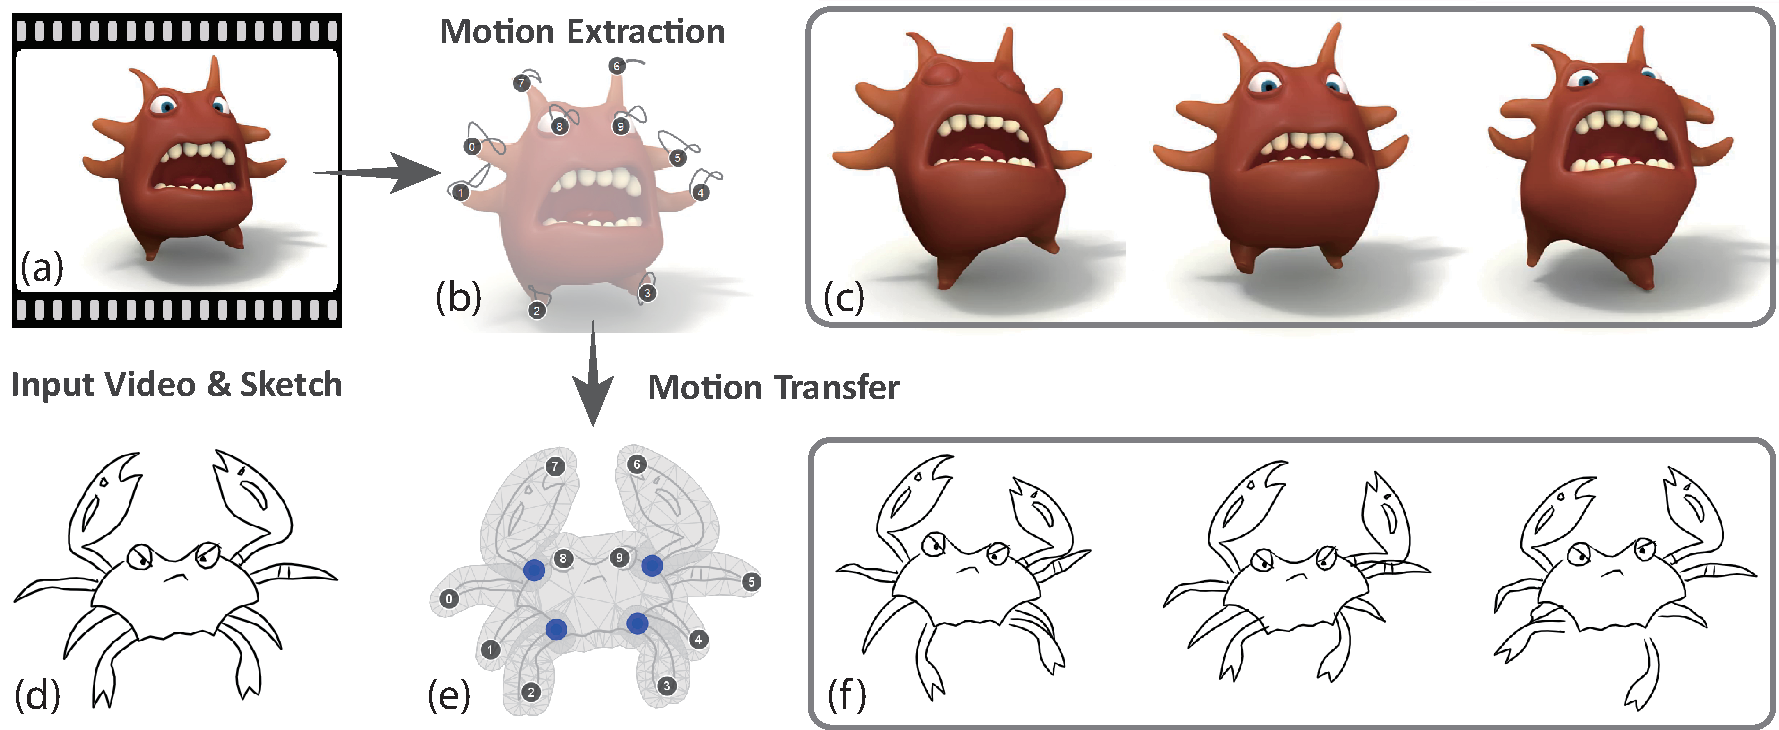
\includegraphics[width=0.8\linewidth]{images/pipeline3}
	\caption{We present {\em Live Sketch}, an interactive system for extracting object motion from a video sequence (top), and transferring it to a static drawing to create vivid 2D sketch animation (bottom).}
	\label{fig:teaser}
}
}
\maketitle


\begin{abstract}
 Sketch animation is a popular art form for depicting object motion in a drawing-in-time way. Creating such animations using traditional tools requires special artistic skills, and is tedious to produce even for trained professionals. In this paper, we propose a new system, \emph{Live Sketch}, \ca{which makes it possible for novice users to create 2D sketch animation} by transferring motion of real objects in videos to static sketch drawings, through an interactive process. By directly transferring object motion from videos instead of creating motion by hand, our system significantly lowers the barrier for creating animations for novice users. Our system addresses a few major technical challenges in this new workflow, such as motion extraction from video, video-to-sketch alignment, and \ca{many-to-one} motion-driven sketch animation. While each of the sub-problems could be difficult to solve fully automatically, we present reliable solutions by combining new computational algorithms with intuitive user interactions. For evaluation, we conduct a pilot study that includes both novice and artistic users. Results show that with minimal training, both types of user are able to generate satisfactory animations using our system with ease. 
\end{abstract}

\category{H.5.m.}{Information Interfaces and Presentation
  (e.g. HCI)}{Miscellaneous} \category{See
  \url{http://acm.org/about/class/1998/} for the full list of ACM
  classifiers. This section is required.}{}{}

\keywords{\plainkeywords}
\section{Introduction}

In recent years, there has been a new wave of research on developing intelligent user interfaces to help novice users create 
artistically expressive sketches and drawings.  Representative examples include \emph{ShadowDraw}~\cite{Lee:2011}, \emph{EZ-Sketch}~\cite{EZSketching:2014}, \emph{ColorSketch}~\cite{Li:2017}, and the repetition autocompletion system~\cite{Xing:2014}. By combining intelligent computational algorithms with intuitive UI controls, these systems enable novice users with little or no formal artistic training to create high quality drawings with minimal user effort, which otherwise cannot be achieved using traditional tools. 



Despite the fact that creating static drawings has been made easier by these tools, creating high-quality 2D animations still remains both difficult and time-consuming.
Traditional animation tools, such as \emph{Adobe Flash} and \emph{Toon Boom} software, require accurate motion keyframing, which is a tedious and labor-intensive process even for experienced artists.
To avoid this, new interactive tools have been proposed to allow artists to specify motion in more creative ways, such as spatio-temporal sketching~\cite{Guay:2015}, or using specially-designed cursive gestures~\cite{Thorne:2004}. Still, using these tools requires not only intensive training, but also  {animation skills} that novice users do not possess.  
Specifically, without intensive training and practice, it is very hard for novice users to mentally map desired continuous object motion to static keyframe drawings that are discrete and sparse.  


In this paper, we present {\em Live Sketch}, a new intelligent interface to assist users to create convincing 2D animation from static drawings using corresponding video examples, as illustrated in Fig.~\ref{fig:teaser}. 
Our main idea  is to extract and transfer object motion from an existing video to a static drawing to animate the character, instead of manual motion specification in the traditional animation workflow. 
The object motion is represented by a sparse set of control points (Fig.~\ref{fig:teaser} (b)) for animation stability and easy user control.
We propose new computational algorithms and combine them with intuitive user controls for robust and controllable motion extraction and transfer.
The main advantage of our system is twofold. First, it enables users with no or little animation 
skills to create animation in an easy-to-control workflow, even for complex non-rigid object motion with self-occlusion. Second, by using semi-automatic tracking and deformation methods, this approach requires much less user interaction compared with traditional tools, and thus can be used for quick prototyping for professionals. 

We address a few major technical challenges using semi-automatic solutions. We  propose a new video tracking approach, which is able to track complex non-rigid object motion and is robust against occlusion and ambiguity. It takes a minimal set of user-specified, semantically-meaningful control points on the first frame, and automatically tracks their positions throughout the video. 
This approach can also incorporate sparse user edits as hard constraints to refine the tracking results in difficult cases. 
In the animation stage, we use mesh-based deformation guided by the tracking results (Fig.~\ref{fig:teaser} (e)) to automatically animate an input sketch, while providing users a set of tools to fine-tune the animation, for instance controlling the local rigidity of the motion. 
We further show how to interactively decompose a sketch into multiple layers to handle complex object motion patterns, such as self-occlusion and topology change. We have evaluated the usability of our system and its support for creativity via a pilot study, leading to very positive results.


Our work presents the following main contributions:
\begin{itemize}
\item The first general, efficient, and user-friendly 2D animation tool that transfers 2D motion from videos to static drawings.
\item A new sparse point tracking method that is robust against occlusion and ambiguity, and allows easy user control (Sec.~\ref{sec:motion_extraction}).
\item A new stroke-preserving mesh deformation method for animating sketch drawings (Sec.~\ref{motion_transfer}).
%\item A set of easy-to-use user tools for fine-tuning the animation (Sec.~\ref{sec:ui}). 
\end{itemize}

\section{Related Work}

%The main approach to free-form motion design is keyframing: character
%poses at specific times are interpolated to produce motion.

\textbf{Digital sketching.} There has been extensive research on how to assist artists or novice users in creating sketches. 
Some methods refine or guide users' sketching by analyzing a crowdsourced set of  images~\cite{Lee:2011}, low-quality drawings~\cite{Gingold:2012}, or even a single image being traced over~\cite{EZSketching:2014}. %improves the sketching quality aided by only a single image.  
%It uses a tracing paradigm and automatically corrects sketch lines that are roughly traced over an image 
%by analyzing and utilizing the image features being traced. 
Xing et al.~\shortcite{Xing:2014} present a painting system that auto-completes tedious repetitions. These methods have focused on assisting users in producing individual static drawings. Animations, on the other hand, rely heavily on users' sense of both space and time~\cite{Sohn:2012,Benard:2013}. Our system aims to relieve users from the tedious control required of motion authoring by making use of video examples.

%\ %---------------------------------------REMOVE LATER------------------------------------------

{\textbf{Sketch-based animation.} Several animation tools with intuitive interaction techniques have been proposed in recent years. A common objective 
	is to develop tools that aid interactive specification of motion 
	trajectories.  Thorne et al.~\shortcite{Thorne:2004} present a set of cursive gestures for sketching a significant 
	variety of motions for 2D characters.
	%Their interface, Motion doodles, interprets motion sketches on the fly to yield interactive animated motions.
	Guay et al.~\shortcite{Guay:2015} introduce a space-time sketching concept that enables animators to create a movement, including shape deformation over time, by sketching only a single stroke.
	Other techniques use predefined motion effects (particle, waves, smoke, etc.) to animate 2D static 
	drawings~\cite{Kazi:2014,Xing:2016}. These methods focus on 
	specific animation effects or a small number of animation styles. 
	Other methods aim at interactively predicting what users might sketch next using temporal 
	coherence~\cite{Wang:2004,Agarwala:2004,Xing:2015}. 
	But they still require many manual sketching operations for each keyframe.
	%\cite{Xing:2015} analyzes all past sketches to predict what the user might sketch next with temporal coherence. 
	Unlike these methods, our \textit{Live Sketch} is able to generate complex non-rigid deformation for a static sketch by retargeting motions from videos with a small amount of user assistance.
}


\textbf{Animation tools using video.} There have been existing tools that also utilize videos for animation creation, as videos provide abundant motion. For example, Ben-Zvi et al.~\shortcite{ben2015line} develop a data-driven method that automatically converts videos and CG animations to stylized animated 
line drawings.  %They maintain temporal coherence by using constrained optimization to build correspondence between tracked points and creating smooth time sheets. 
Kyprianidis et al.~\shortcite{Kyprianidis:2013} survey non-photorealistic rendering techniques that transform images and videos into artistically stylized renderings.
These methods focus on changing the rendering styles of input videos instead of extracting the underlying motion for animating new line drawings. 

Animations can also be created by tracking a contour of an object in the video and using its temporally coherent information.
For instance, Bregler et al.~\shortcite{Bregler:2002} track the motion from traditionally animated cartoons and retarget it onto 3D models or 2D drawings.
It takes a keyframe-based approach and requires series of corresponding input and output key shapes for deformation interpolation. In contrast, we take non-keyframe-based approaches to require only a single static drawing as input, which is easier to prepare.
Their method further requires a sub-part decomposition procedure, which is relatively easy for cartoon characters but is hard for real video objects. 
% It parameterizes cartoon character motion into global affine transformation and a series of input key shapes as deformation basis, which are picked by the user. However, given the complexity of real-world object motion, it is unclear how to intuitively construct the key shapes. 
Agarwala et al.~\shortcite{Agarwala:2004} present a rotoscoping approach that uses computer vision techniques to reduce user interaction in the contour-tracking process. 
The extracted contours from this system can be used to drive user sketches for video stylization. 
Our system uses sparse control points as motion representation, which are much easier to track accurately than contours, and thus requires much less computation and user intervention in the tracking process.

\textbf{Face and body driven animation.} 
Our system is closely related to automated human-performance-driven animation. 
MoCap~\cite{Kitagawa:2008} is the industry standard for capturing 3D human pose for animation. It requires complicated hardware setup that is not easily accessible to normal users. 
Fitting 3D face or body models to images and videos to extract human motion has been extensively studied~\cite{Chen:2012,Cao:2013,thies2016face,posemachine,Reinert:2016}. It has enabled new real-time face- or body-driven animation systems such as Adobe Character Animator. 
Park et al.~\shortcite{Park:2006} directly synthesize human motion in video by analyzing exemplars.
However, these systems are limited to facial expression or body motion only. In contrast, our system is designed as a general animation tool that can handle a wide range of objects. Furthermore, it uses a regular video as motion source, which is relatively easy to capture and vastly available online. 

\textbf{Cross-modality motion retargeting.}
Many systems have been proposed to transfer motion across different modalities. 
Hornung et al.~\shortcite{Hornung:2007} transfer 3D motion data to 2D image objects. 
Diener et al.~\shortcite{diener:inria-00389326} retarget 2D motion fields for the animation
of 3D plant models.
Zhou et al.~\shortcite{Zhou:2005} propose to use the volumetric graph Laplacian for large 3D mesh deformation, allowing motion to be transferred from exaggerated 2D animations to 3D meshes.
Our system is a pure 2D system, and thus is applicable even when 3D models are not available.

\textbf{Video tracking.}
Previous single object tracking methods~\cite{Martinez:2008,Artner:2011,Cehovin:2013,Cai:2014} often utilize weak local features of sampled patches to track a single object at the bounding box level. 
The box position is determined from all patches through a voting or statistical aggregation method. Our application however requires more than a bounding box; it requires tracking sparse control points to capture major structural deformation. 

Sparse feature tracking is a fundamental component for video analysis that has been extensively studied in the computer vision literature.
Our tracking method is built upon well-known tracking techniques such as good-feature-to-track~\cite{Shi_1994_3266} and Struck~\cite{6126251}. However, most previous tracking methods track each feature point individually without considering their geometrical relationships. This is valid for most computer vision tasks where hundreds of features are being tracked on each frame, and tracking errors are eliminated by outlier removal methods such as RANSAC. However, since we only track a few semantically-meaningful control points, tracking failure of a single point would result in large distortion.
This problem is alleviated by our new motion extraction method. 
%\hongbo{In-betweening techniques can also be briefly discussed:
%Re-using traditional animation: methods for semi-automatic segmentation and inbetweening;
%Betweenit: An interactive tool for tight inbetweening}


%Kyprianidis: focusing on non-photorealistic techniques for transforming 2D input (images and video) into artistically stylized renderings
%. First, the fusion of higher level computer vision and NPR, illustrating the trends toward scene analysis to drive artistic
%abstraction and diversity of style. Second, the evolution of local processing approaches toward edge-aware filtering for real-time
%stylization of images and video. 

%\textbf{Motion retargeting techniques.} Motion retargeting aims to transfer the motion from one source to another. It usually focuses on specific class by using existing motion or predefined tracking model, such as character, fluid, animal gaits, face, etc. Our system is proposed to transfer the extract motion from the non-rigid deformed object in a video to a sketch and they can belong to any class and be different.

\section{Our System}

\subsection{System Overview}\label{sec:overview}

{\bf Inputs.}
As illustrated in Fig. 1, 
our system takes as input a static sketch drawing represented as a {\em vector graphics}, and a video sequence that contains desired motion of a moving object for the sketch. The moving object should be entirely visible throughout the video. For minimal user interaction, the video object should contain relatively rich texture and has a clear boundary against the background. Let's first assume that the user-provided sketch drawing matches the video object well in shape, so that the correspondence between image features and sketch lines exist naturally. Such sketches can be easily created with one of the video frames as reference by using previous image-guided sketching interfaces like EZ-Sketching~\cite{EZSketching:2014}. We will describe in Sec.~\ref{sec:cp_transfer} how to extend the system to handle more creative user sketches that have larger shape deviation from the video object.  

{\bf Motion Representation.}
A key question for our motion transfer task is the representation of object motion. Given the complexity of natural object motion, it is difficult to describe it using parametric forms, as similarly done in \cite{Bregler:2002}. For non-parametric representation, we could choose either dense or sparse motion flow. The former can be extracted by optical flow methods, while the latter be computed by using sparse feature tracking. 

We have experimented with both representations, and concluded that sparse feature point trajectories are more suitable for our task. The reason is that dense flow often contains tracking errors that could distort the sketch during animation, and these errors are hard to correct through a user interface, given that motion is defined on every pixel. 
On the contrary, sparse trajectories allow us to enforce strong spatial and temporal smoothness in motion, resulting in more stable animation. It further allows quick user editing by interactively moving the positions of these points. The downside of using sparse representation is that motion with finer granularity cannot be captured and transferred. This problem, however, can be partially alleviated by adjusting the spatial distribution of control points, as described in Sec.~\ref{feature_extraction}.

\if 0
\paragraph{Workflow}

Our system workflow is shown in \ca{Fig.~\ref{fig:pipeline}}. 
Given the input video and sketch drawing, our system first  extracts \hongbo{user extracts?} a series of control points that satisfy two constraints: (1) be easy to track; and (2) be semantically meaningful to guide the sketch deformation to create animation, with the user's help. We then construct an elastic graph using these points as nodes, and track their positions through the video using a novel graph tracking method that jointly considers (1) the tracking accuracy of individual nodes; and (2) the elasticity or rigidity constraints defined on edges between nodes. Given that perfect tracking could be extremely difficult for hard cases, we keep the user in the loop in the tracking process to provide additional guidance. The user can correct tracking errors on keyframes, or specify special geometric constraints between any pair of nodes. The algorithm takes into account the user inputs to produce satisfactory tracking results. 
Finally, the tracked control points are used as guidance to a stroke-preserving mesh deformation algorithm to generate a deformed sketch on each frame, resulting the final animation. 
We further allow the user to quickly specify local rigidity of mesh deformation for achieving more desirable results. 
%\qingkun{However, some strokes may be distorted by the direct mesh deformation. Therefore, we allow the user to select the strokes by a local rigidity brush. Our system then reconstruct the mesh by adding more triangles which is used for keeping the shape of these strokes. Our method does not add the shape constraint to all strokes because the harder the shape constraint we give, the more motion would be lost.}
In the following sub-sections, we will describe each of the technical components in more detail. 
\fi
%
%\begin{figure}
%	\centering
%	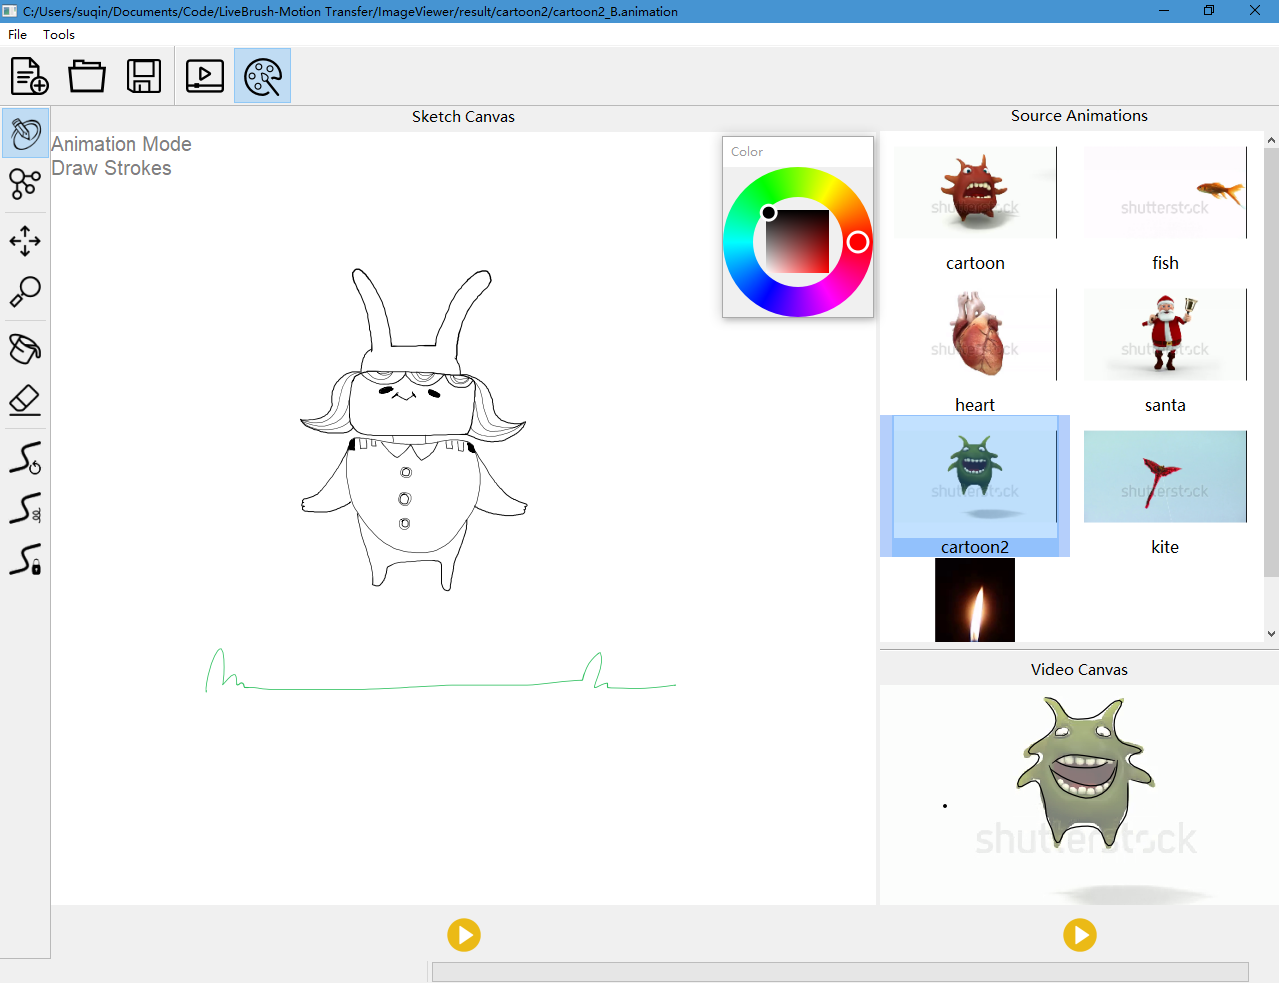
\includegraphics[width=0.85\linewidth]{images/ui}
%	\caption{}
%	\label{fig:ui}
%\end{figure}


\subsection{User Interface} \label{sec:ui}
The workflow of our system contains two stages: (1) {\em motion extraction} from the input video; and (2) {\em motion transfer} to the sketch. We first introduce the user interfaces for these two stages, as shown in Fig.~\ref{fig:ui2}.
%\begin{figure}
%	\centering
%	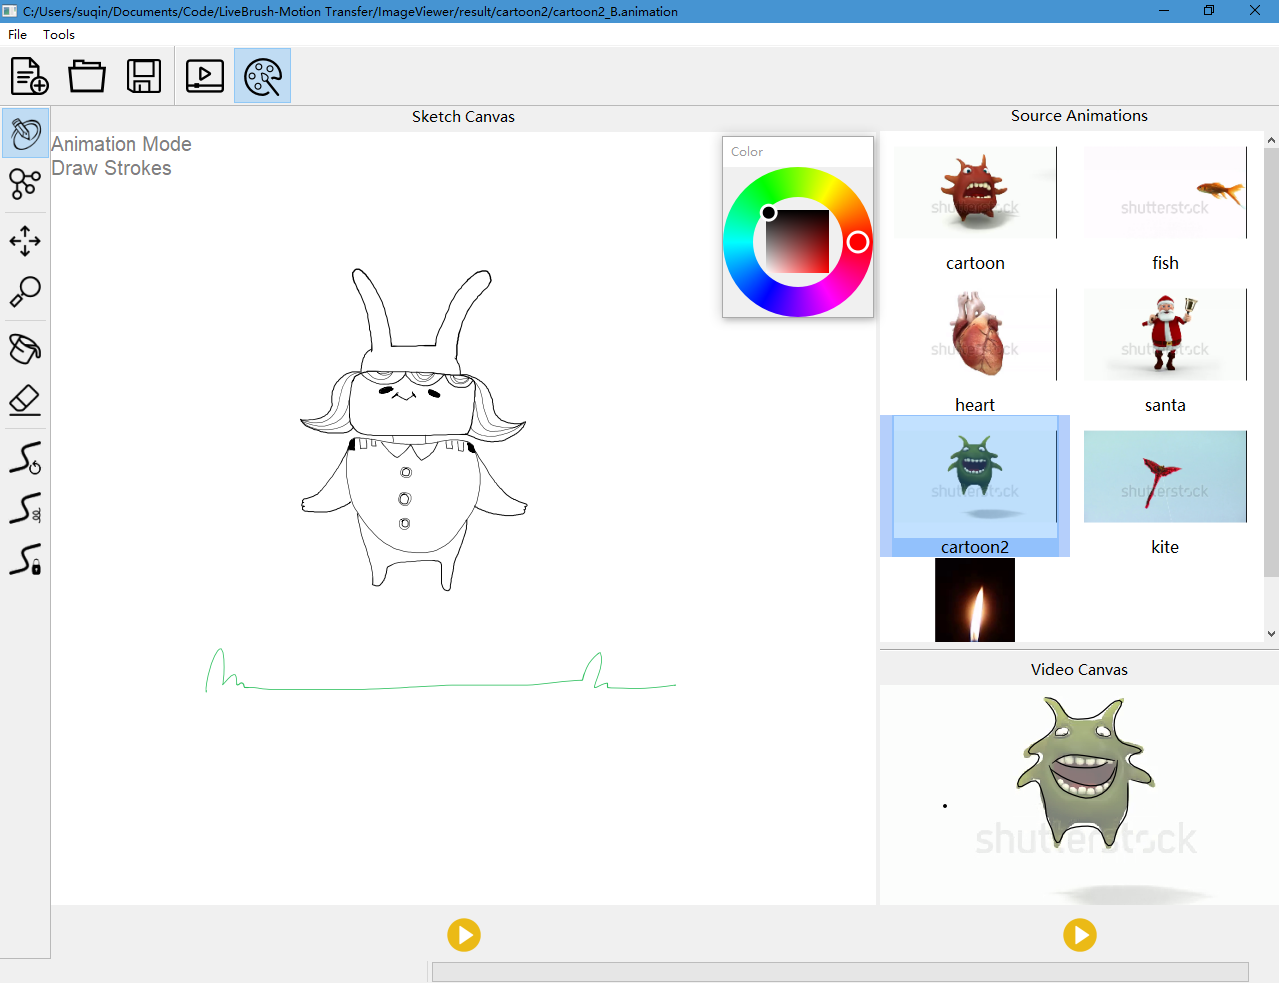
\includegraphics[width=\linewidth]{images/ui}
%	\caption{User interface of our system.}
%	\label{fig:ui}
%\end{figure}

\subsubsection{Motion Extraction}\label{sec:motion_extraction}

After loading a new video into our system, 
the user first roughly specifies the desired object on {one of the video frames (the first frame by default)}, from which motion will be extracted.
The system suggests an object outline by applying automatic GrabCut segmentation~\cite{Rother:2004}, which works well when the background is clean. Otherwise, the user can quickly draw the correct outline using a pen tool. The extracted object shape will later be aligned with the user-provided sketch for motion transfer.

In the next step, the user defines a set of structural control points inside the object, which are automatically tracked through the entire video. The details about control point extraction are described in Sec.~\ref{feature_extraction}, and our tracking method is described in Sec.~\ref{sec:motion_extraction}.  
The trajectories of these control points represent the object motion, and will be applied to the corresponding control points on the sketch for animation. 
Given that tracking is not always perfect, our interface also provides manual tools for fine-tuning the extracted motion by adding, removing or adjusting the control points. The motion trajectories are updated in real time and visualized to the user during the editing process (see Fig.~\ref{fig:ui2}, Left). 
%A screen shot of this interface is shown in Fig.~\ref{fig:user_interface}.
\begin{figure}
	\centering
	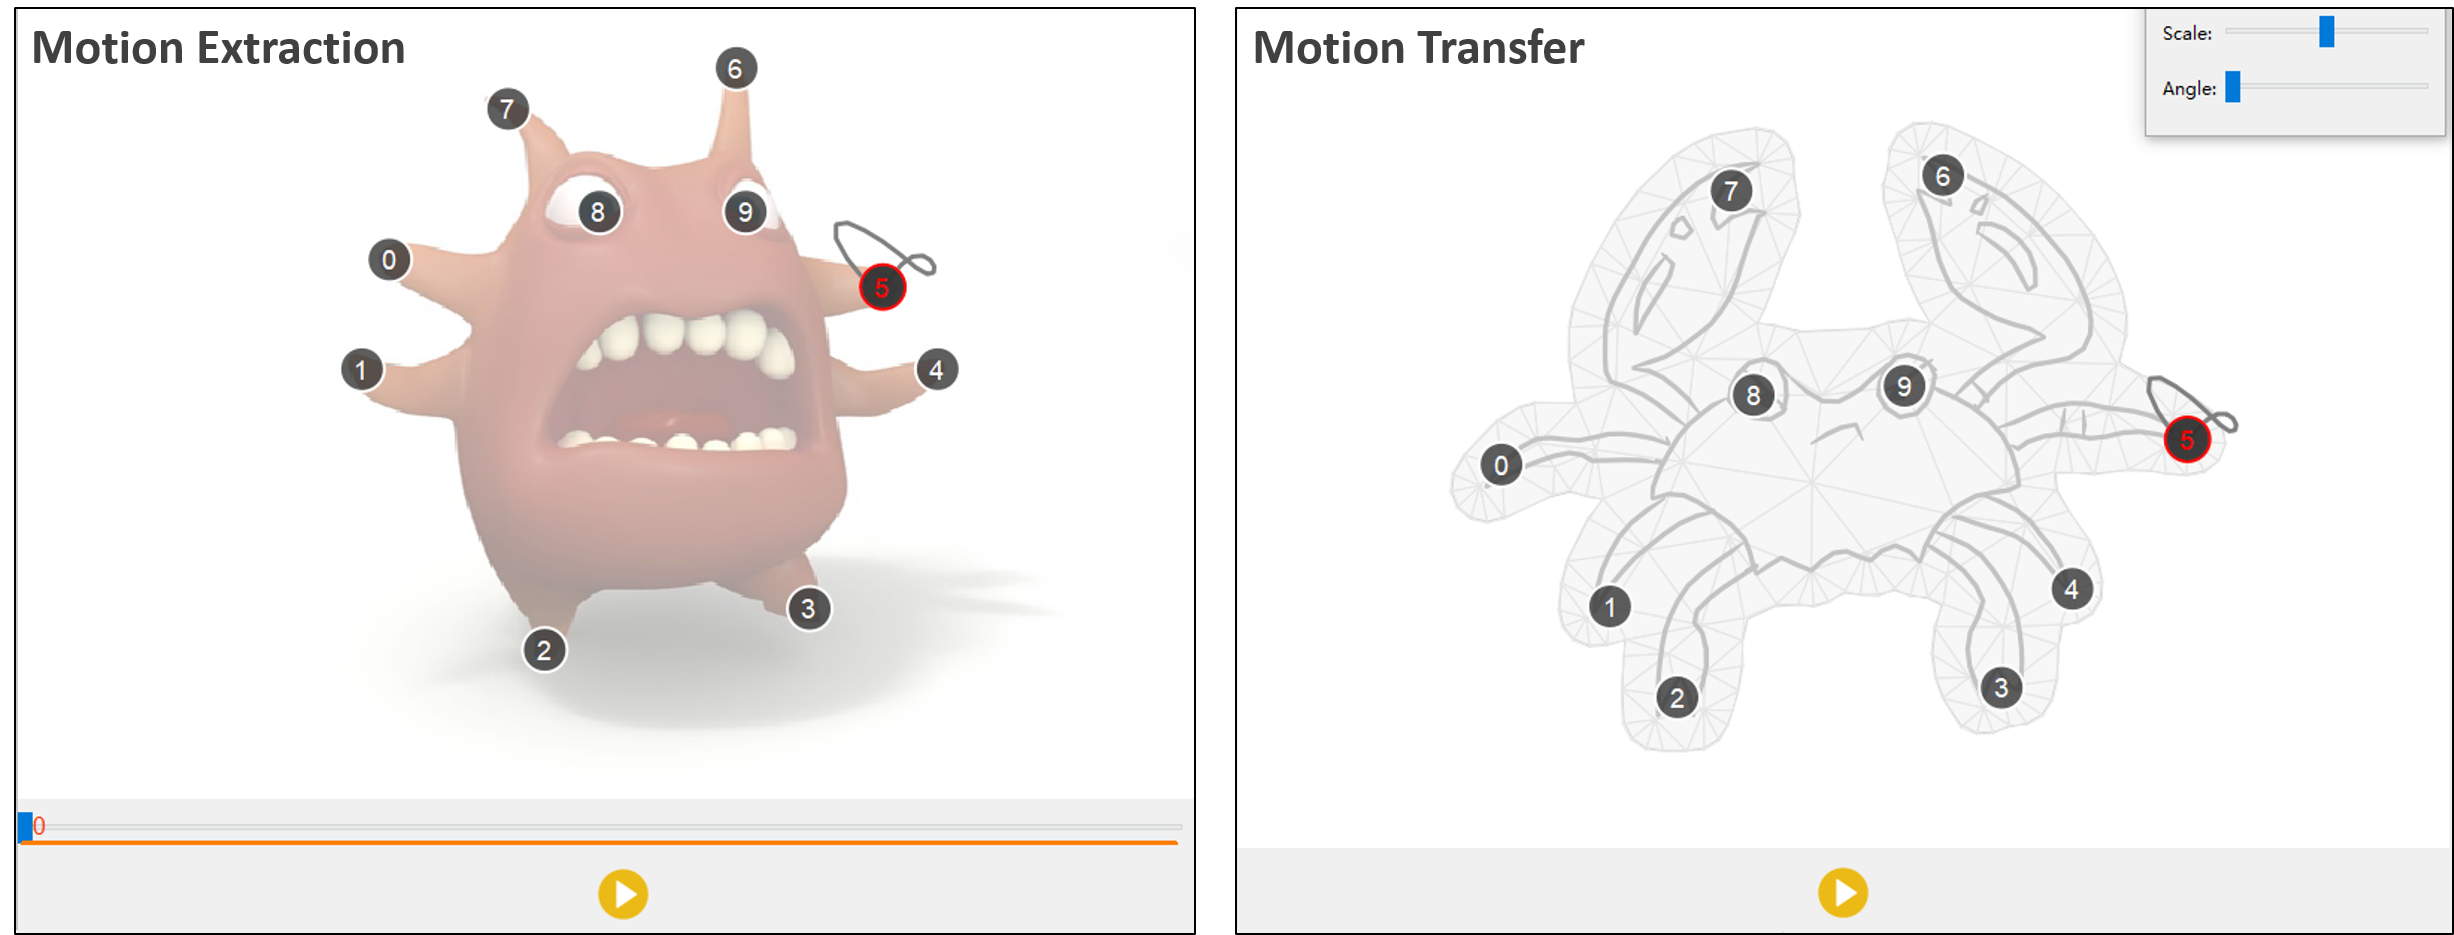
\includegraphics[width=\linewidth]{images/ui2}
	\caption{Our user interfaces. Left: motion extraction UI, where control points are defined and tracked in the input video. Right: motion transfer UI, where the position and motion of the control points are used to drive the sketch. The corresponding control points on the video and sketch are labeled with the same numbers.}
	\label{fig:ui2}
\end{figure}

\begin{figure}
	\centering
	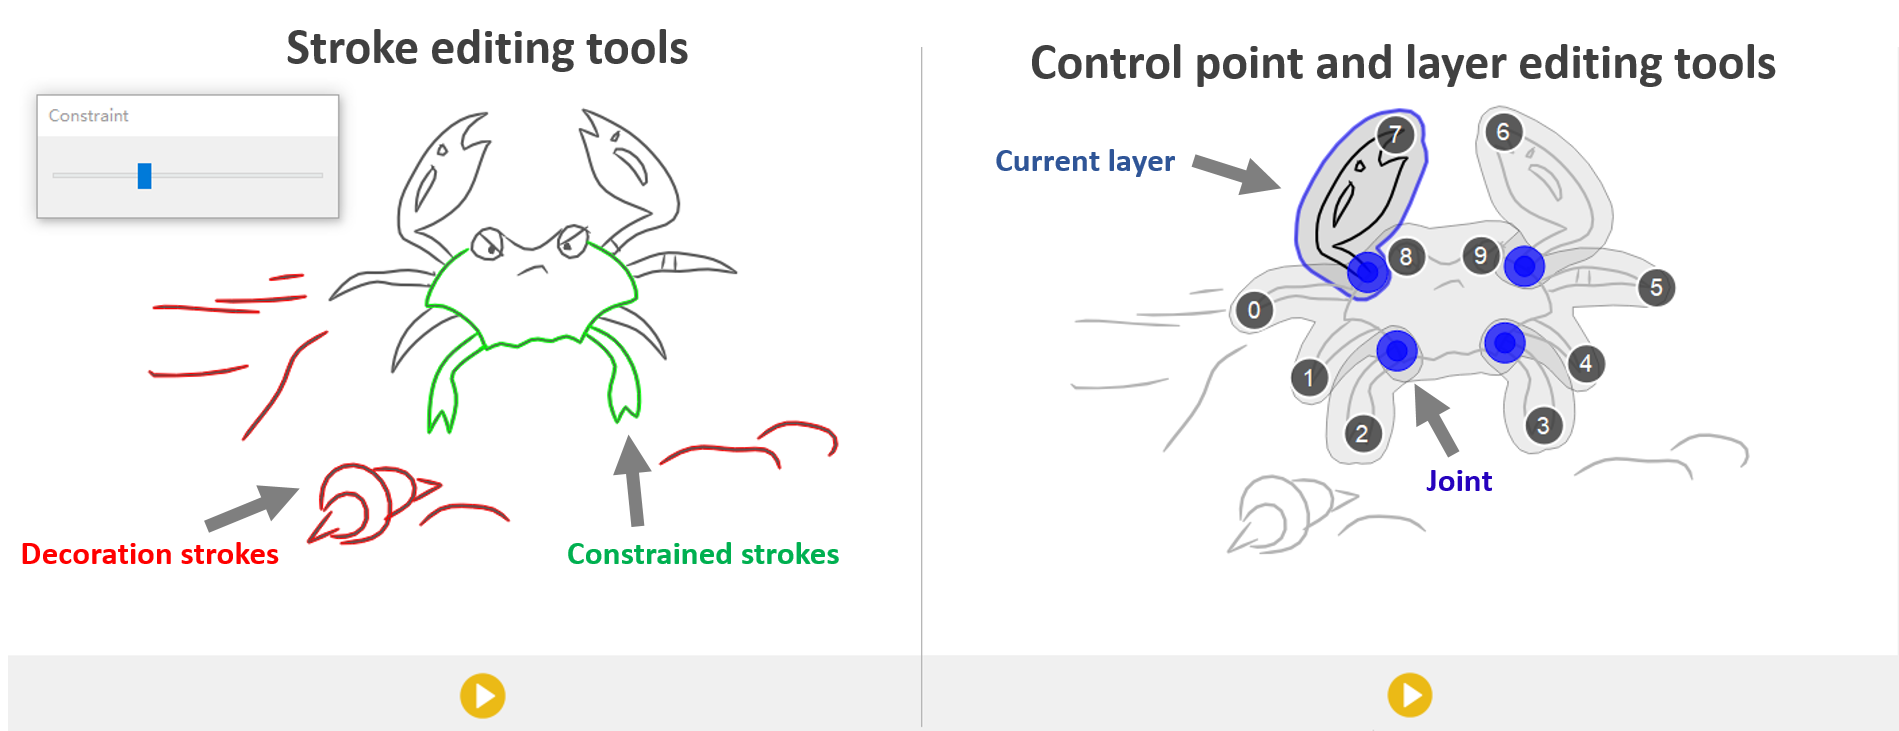
\includegraphics[width=\linewidth]{images/othertools}
	\caption{Interactive tools for motion transfer. Left: the user can label selected strokes as decoration strokes (i.e., no motion), or add strong shape rigidity constraints to strokes. Right: the user can group several strokes as a new layer to animate them independently from other strokes, or add/move automatically initiated joints in the layer intersection regions. }
	\label{fig:othertools}
\end{figure}

\subsubsection{Motion Transfer}
As the target for motion transfer, the user either imports an existing sketch or draws a new one in our system.
The system automatically computes shape correspondence between the video object and the user-provided sketch, in order to map the control point trajectories to the sketch (Sec.~\ref{sec:cp_transfer}). These mapped control points are used as constraints in a mesh deformation process to drive the animation, as detailed in Sec.~\ref{motion_transfer}. The user can immediately review the animation result without any additional manual operation.

Our interface also provides interactive tools for fine-tuning the automatically-generated sketch animation, as shown in Fig.~\ref{fig:othertools}. 
First, it allows the user to adjust the spatial positions of the control points on the sketch, which are automatically inferred from the control points on the video object. 
% User first select one edit the spatial correspondence between sketch and video by two control points 
%First, our system shows a set of control points for user to do the animation editing. User can move the control points to change their influencing regions.
Another useful tool is ``Rigidity Stroke'', which can be used to prevent local shape distortion during the animation.
The user can also use a ``Static Stroke'' to mark sketch components that are to remain stationary, like those for background decoration.

One important feature of our system is its ability to decompose a sketch and animate it in multiple layers (see Fig.~\ref{fig:othertools}, Right). This is particularly useful for handling self-occlusions, which are common for video objects with complex motion. To create such layers, the user can use a ``Layer Brush'' to paint over strokes that should be grouped together, based on the semantics of the object and its motion. We also provide an interface for users to refine the automatically generated joints between layers to fine-tune the animation. Please refer to Sec.~\ref{sec:multi-layer_animation} for more details.
% The user can additionally add or move joints' positions if needed to fine-tune the animation.



\subsection{Control Point Extraction}\label{feature_extraction}

In our system, object motion is represented by a set of sparse control points which are tracked through the video, and used as constraints for deforming the sketch for animation. We have done extensive studies on automatically computing these points. 
We have tried to use image features such as SIFT or SURF to find good points to track, and also explored determining the points based on the initial object shape. 
In the end we conclude that although these automatic approaches do work well in some cases, they cannot handle a wide variety of examples well. This is because we have a set of strict requirements for these control points:
\begin{enumerate}
\item They should be sparsely distributed across the entire object shape to capture its shape characteristics.
\item They should be easy to track in the video.  
\item They should obey the semantics of the object, e.g., respecting semantic symmetry.
\item Their distribution should respect the motion characteristics of the object. For example, one control point could be enough for a flying baseball; however more are needed for a fly bird to capture its wing motion. 
\item The number of control points should be minimal for easy user adjustment.
\end{enumerate}

It is relatively easy to satisfy Requirements 1, 2 and 5, as they only require local image feature and shape analysis. However, without deep semantic understanding of the object and its motion, it is very difficult for automated algorithms to satisfy Requirements 3 and 4. 
On the other hand, it is relatively easy for the user to preview the video and determine the semantics of the object and its motion. 
We thus resort to a manual procedure for specifying control points. We propose a few general guidelines for doing so: (1) distribute the points sparsely to cover the whole object; (2) for symmetric object parts, specify points in roughly the same configuration; (3) place no more than 20 points for general objects. We do not explicitly ask the user to specify points that are easy to track, which is hard for the user to do. Instead we employ a robust tracking algorithm that jointly optimizes all tracking points, as detailed in the next section. 

{\bf Discussion.} Note that the distribution of the control points determines the granularity of the motion we extract. Fewer control points results in coarser motion, and vice versa. However, having too many control points is also problematic, as the tracking failure would increase, and the motion field becomes less stable due to tracking errors. Given that we will enforce temporally-smooth motion fields for animation stability, we have found that a smaller set of control points (one or two dozens) is usually sufficient for a wide variety of examples. 

\if 0 
The first step of the system is to extract a set of sparse points on the sketch as ``knobs'' for deforming the sketch for animation. The position of these points are tracked through the video, so object motion is represented by their trajectories. Note that since the primary utility of these points are for controlling animation, commonly used image features such as SIFT or SURF are not desirable, as they describe only local image features rather than semantically meaningful representation of the the object shape. Furthermore, we expect the number of such points to be minimal for reduced tracking complexity and smooth sketch deformation. 
Automatically computing such points is extremely hard, as it requires strong prior knowledge on the motion of the underlying physical object. 

We first compute the object region that the control points should be extracted from. This is done by applying the active contour method~\cite{Kass88snakes} on the sketch image to produce an membrane that encloses all sketch strokes.
Inside the object region, we find all the starting and ending points of the strokes, as well as high curvature points along each stroke. These points encode most of the topology information of the sketched object. We group them into clusters based on their spatial distances by using a simple K-Means clustering in 2D space, and use the centroid of each cluster as a control point candidate. The user can additionally move or delete these points, or adding new ones through our interface. 

\ca{\sout{ The user-adjusted control points can well represent the structure of the object, but may not be optimal for tracking. To improve their trackability through the video, we apply a final adjustment step to their positions. 
For each control point, we use the multi-level Shi-Tomasi corner detection method~\cite{Shi_1994_3266} in its vicinity to compute a local multi-level ``goodness to track'' measure, where the size of the support region in each level, denoted as $r$, is set to be $ r_0, 2r_0, 3r_0 $, with $r_0$ being the 1/10 diagonal length of the sketch bounding box. We then identify the local maximal in this multi-level local measurement map, and move the control point to it. We also record the support region size for each adjusted control point, which will be used in the tracking process. Formally, we describe the supporting image region of a control point as $C_i=\{\mathbf{x}_i, r_i\}$ (i.e., center position and size). $r_i$ is kept as a constant and we seek to determine $\mathbf{x}_i$ in each frame in the tracking process. 
}}

\qingkun{Because I only used one patch level (0.075 diagonal length of the video) in tracking part, so here we only use one patch size for point extraction.}

\fi
\subsection{Motion Extraction}\label{sec:motion_extraction}
After specifying the control points, we track their positions throughout the video.
A na\"{i}ve approach would be to track each control point individually using standard point tracking methods, e.g., KLT point tracker~\cite{yilmaz2006object}. 
However, these methods may fail for some points that are hard to track, e.g., points specified in textureless regions, resulting in drifting. Used as hard constraints, these drifted points will later distort the sketch shape in the final animation.
Given that automatic tracking failure may always occur no matter how robust the underlying algorithm is,  
we employ an interactive tracking procedure. We first adopt the dynamic-programming-based trajectory optimization framework~\cite{Amberg:2011,Buchanan:2006} to track individual points, which is quite efficient and can provide near real-time feedback to the user. 
When tracking failure occurs, the user only needs to modify the tracking position of a failed point on a particular frame, and this method can use it as a hard constraint to globally refine the whole trajectory. Therefore, the user can quickly refine the tracking results by only editing a few frames.

Specifically, the tracking algorithm optimizes the following energy for each feature trajectory:
\begin{equation}\label{eq:tracking}
E_{tr}(\textbf{x}) = \sum_t\lambda_d d(\textbf{x}_t, \textbf{x}_{t-1})+\lambda_u u(\textbf{p}_t,\textbf{p}_{t-1})+\min_k(a(\textbf{p}_t,\textbf{c}_k)),
\end{equation}
\ca{where $ \textbf{x}_t $ represents the position of the control point on frame $t$, and $ \textbf{p}_t $ denotes the feature descriptor of the image patch centered at $\textbf{x}_t$. The energy includes three parts. The velocity term $ d(\cdot)=\|\textbf{x}_t - \textbf{x}_{t-1}\|^2_2 $ and update penalty term $ u(\cdot)=\|\textbf{p}_t - \textbf{p}_{t-1}\|^2_2 $ measure the motion intensity and appearance variation between two consecutive frames, to achieve a smooth motion and appearance transition. The third term $ a(\cdot) = \|\textbf{p}_t - \textbf{c}_k\|^2_2 $ is a measure of the appearance deviation from the user-specified control point locations $ \{\textbf{c}_k\} $. User may manually specifies two or more control point positions at different frames. We measure the appearance energy of points at other frames using $ \min_k(a(\textbf{p}_t,\textbf{c}_k)) $, so that they should match at least one of these $ k $ control points. }
The optimization is mainly divided into two stages: preprocessing using k-d tree and trajectory optimization based on dynamic programming. More details of this method can be found in~\cite{Amberg:2011,Buchanan:2006}.

Built upon this algorithmic framework, we further improve the tracking method by addressing two common problems that lead to drifting: occlusion and ambiguity. These additional components, as detailed in the next two sections, allow our tracking method to perform more reliably than previous ones on tracking complex object motion with topology changes. 


\subsubsection{Occlusion Handling}
% \hongbo{Qingkun: check if this part is our contribution or not}
Occlusion has been considered by many existing automatic tracking methods. However, it still leads to serious drifting in difficult cases. There exists no good user interface for correcting drifting other than manually editing results frame by frame.
Following~\cite{Amberg:2011}, we modify the graph used for dynamic programming by adding extra edges from each control point to all points on the next few frames. When occlusion happens, the optimization favors a trajectory that passes through the extra edges, thus skipping a few frames where occlusion occurs in.
In our system, the skipped/occluded part of the trajectory is interpolated using Hermite interpolation for smooth animation. 
%as tracking errors of individual control points often lead to significant distortion of the sketch image. Such an example is shown in Fig.~\ref{fig:distortion}, where \ca{XXX}


\subsubsection{Ambiguity Handling}\label{sec:ambi}

Another source of drifting is ambiguity, i.e., when two or more tracking points with similar appearance get close to each other. An example is shown in Fig.~\ref{fig:ambiguityhandling}. When the two legs of the tiger cross, the two control points become too close to each other, and they end up tracking the same image feature going forward, resulting in a collide.  

To solve this problem, we propose a new energy minimization method to jointly optimize the tracking results of multiple points together. 
The main idea of this method is that instead of tracking a single trajectory for each point individually, we first generate a set of trajectories for each control point as candidates, and then employ a global optimization approach to select the best one for each point, by jointly considering multiple points together.

{\bf Candidate Trajectories.}
Given all control points on a keyframe, we first compute the appearance similarity between any two points, based on the image patch color distance centered around them (we use $9\times 9$ patches). We then group points into several sets, each containing the points that have similar appearance. Denote one such set  as $S=\{\textbf{x}^1,...,\textbf{x}^n\}$. For each point $\textbf{x}^i$,
we apply the method proposed in~\cite{chondrogiannis2015alternative} to compute a set of candidate tracking trajectories. This method has two major parameters: (1) the maximum overlap between any two candidate trajectories, which we set as $T/4$, where $T$ is the total number of frames; and (2) a tracking cost threshold. We then sort the candidates based on their tracking costs (computed in Eq.~\ref{eq:tracking}).

{\bf Trajectory Optimization.}
In the next step, we find the best trajectory for each point by  jointly optimizing over multiple tracking points.
This can be formulated as the following energy minimization problem:
\begin{equation}\label{key}
\arg \min \sum_{i}E(\textbf{x})= \arg \min \sum_{i} (E_{tr}(\textbf{x}) + \beta \sum_{j \neq i} E_o(\textbf{x}_{i}, \textbf{x}_{j})),
\end{equation}
where the tracking energy $ E_{tr}(\textbf{x}) $ is measured by Eq.~\ref{eq:tracking}. $ E_o({\textbf{x}_{i}, \textbf{x}_{j}}) $ is defined as the normalized duration of the overlapping portion of the two trajectories. Intuitively, this term prevents two similar control points to collapse into a single one, in which case the overlapping portion of the two trajectories will be large. 

We use a greedy algorithm to minimize this energy. 
We first initialize the solution by choosing the trajectory that has the minimal tracking energy for each point. We then find the point that has the largest total energy according to Eq.~\ref{key}, and select another candidate trajectory that can best minimize this energy. We repeat this process until the total energy cannot be further reduced. 

\begin{figure}
	\centering
	\includegraphics[width=\linewidth]{images/ambiguityhandling2}
	\caption{Solving tracking ambiguity using multi-track optimization. Top: four control points defined on the four legs collide when the legs cross, due to appearance ambiguity. Bottom: our new tracking method proposed in Sec.~\ref{sec:ambi} can effectively prevent such cases.}
	\label{fig:ambiguityhandling}
\end{figure}


%Then 
%compute the overlapping ratio between each point pair $ (i, j) $ based on current optimal . We let the ratio as .
%Denote the optimal trajectory candidate of each point as $ \textbf{p}^*_i $. We first initialize it as $ \textbf{p}_{i1} $, which has minimum tracking cost, but may have large overlapping with other points.
%\paragraph{Overlapping Detection}
%%Before tracking, we first compute the similarity between all objects that are specified manually by the user based on patch descriptor (we use SURF feature in our implementation). 
%
%Given a set of similar points, they may overlaps with each other during the tracking. We first obtain their trajectories $ \{\textbf{p}\} $ by tracking each point individually. Then for each pair of trajectory $ \textbf{p}^a $ and $ \textbf{p}^b $ of two keypoint $ a $ and $ b $  of this set, we compute their closeness at each frame by: 
%\begin{array}\label{eq:closeness}
%C(p^a_f, p^b_f) = \alpha\lVert p^a_f-p^b_f \rVert^2_2 + (1-v^a_f \cdot v^b_f),
%\end{equation}
%where $ v^a_f$ and $ v^b_f $ are the normalized vector of $ \overrightarrow{p^a_{f-1}p^a_f} $ and $ \overrightarrow{p^b_{f-1}p^b_f} $. The first term represents their Euclidean distance and the second term represents their direction consistency. 
%The equation implies that the two trajectories are close only when their distance is small and their direction is same.
%When $ C(p^a_f, p^b_f) \leq \epsilon$, the two trajectories are flagged as overlapping at the $ f $th frame.
%
%Based on this measurement, we count the overlapping frames, which is denoted as $ C(p^a, p^b) $.
%%Based on this measurement, we denote the overlapping time interval $ I=[n, m] $ when overlapping happens between $ n $th and $ m $th frame. To tolerate instant overlapping, we only considers the overlapping intervals with length larger than 3, i.e. $ m - n>=3 $.
%$ \alpha $ and $ \epsilon $ are set 0.02 and 3.0 in our implementation.
%Finally, we can obtain a set of overlapping intervals between each pair of trajectories. 
%
%%Then an overlapping detection is run between each similar object pair after we obtained the trajectory using graph tracking for each object. Given one point pair $ p_i,q_i $ of the two trajectories $ \textbf{p},\textbf{q} $, , the intesection parts are detected based on the following equation:
%%\begin{equation}\label{key}
%%f(p_i, q_i) = \alpha\lVert p_i-q_i \rVert^2_2 + (1-u_i \cdot v_i),
%%\end{equation}
%%where $ u_i$ and $ v_i $ is the normalized vector of $ \overrightarrow{p_{i-1}p_i} $ and $ \overrightarrow{q_{i-1}q_i} $. It means two trajectories overlapps at $ p_i $ and $ q_i $ only when their distance is small and their direction is similar.  $ \alpha = 0.02 $ in our implementation.
%%Then when $ f(p_i,q_i) \leq 3$, it means the two trjactories $ \textbf{p} $ and $ \textbf{q} $ overlap at the $ i $th frame.
%
%\paragraph{Overlapping Removal}
%Next we run the overlapping removal for each of the overlapping intervals one by one in time order.
%First, for each similar point set, we sort all overlapping intervals by their starting time. Then the intervals will be removed according to this order.
%
%Given the first interval $ I=[n, m] $, we modify the edge weight of keypoint $ a $'s graph in the overlapping interval by
%%Because we assume that there is no long common consecutive trajectory parts shared by two objects, we need to remove the overlapping when a long sequence of overlapping frames exists.
%
%\begin{equation}
%\begin{array}{rcl}
%w(e) & = & +\infty \text{ if }C(e) < \epsilon\\
%C(e) & = & \alpha\lVert p^a_f-x_f \rVert^2_2 + (1-v^a \cdot v^e) 
%\end{array}
%\end{equation}
%
%$ e_f=(x_f,y_g) $ is an edge in keypoint $ b $'s graph from the $ f $th to the $ g $th frame, $ v^e $ is the normalized vector of $ \overrightarrow{xy} $ and $ v^a $ is the normalized vector of $ \overrightarrow{p^a_f p^a_g} $.
%The reweighting makes sure that there is no tracking path passing though the overlapping parts. 
%Then we update the part of $ a $'s trajectory, which starts from frame $ m $ based on $ a $'s reweighted graph to the end. Denote the new trajectory as $ \textbf{q}^a $. We also reweight keypoint $ b $ graph using similar way and update $ b $'s trajectory, which is denoted as $ \textbf{q}^b $.
%If the cost of $ \textbf{q}^a $ is smaller than $ \textbf{q}^b $, we set the trajectory of $ a $ as $ \textbf{q}^a $ and keep the $ b $'s trajectory unchanged, i.e. the two trajectories become $ \textbf{q}^a, \textbf{p}^b $.
%Otherwise, we set $ b $'s trajectory as $ \textbf{q}^b $ and keep $ a $'s trajectory unchanged. Their trajectories become $ \textbf{p}^a, \textbf{q}^b $. Obviously, because of the reweighting scheme, there is no overlapping between their new trajectories in both scenarios during the interval $ I=[n, m] $. Therefore, one overlapping interval is removed. 
%
%We recompute the overlapping status among the new trajectory set and obtain the new first interval $ I'=[n', m'] $. 
%Note that $ [n,m] $ is the first appeared overlapping interval before and the second pass does not change the positions of the trajectories between the interval $ [1,n] $. Therefore, the overlapping status between interval $ [1,n] $ does not change, i.e. no overlapping exists in $ [1,n] $ and $ n'> n $. It ensures that the overlapping intervals can be removed one by one according to the time order.
\subsection{Control Point Transfer}\label{sec:cp_transfer}
To transfer the extracted motion to the input sketch, we first need to map the control points specified on the video object to the sketch. This is done by aligning the sketch with the video. More specifically, we apply the Shape Context method~\cite{belongie2000shape} to build correspondence between the sketch image and the extracted object contour as described in Sec.~\ref{sec:motion_extraction}. For a control point inside the video object, we represent its location using barycentric coordinate of a set of evenly sampled contour points, and compute its location using the same barycentric coordinate on the sketch image. 
For sketches drawn over a keyframe using an over-painting interface similar to the EZ-Sketching system~\cite{EZSketching:2014}, the alignment step is optional, since the sketch is already well aligned with the underlying image.

%Thus the control points extracted from the video can be directly applied to drive the sketch animation. 
%


\subsection{Motion Transfer} \label{motion_transfer}

After tracking is done, we use the sparse control point trajectories to drive the final sketch animation. 
For this purpose, we first embed the sketch into a mesh and then use a mesh deformation method to warp the mesh for animation. The mesh is generated by
triangulating an expanded region of the sketch (see Fig. 1).
Our expectation for the deformation is twofold: 
(1) the deformed mesh should closely follow the guidance of the control points to preserve the extracted motion; 
and (2) the original sketch strokes should not be distorted too much to avoid unnatural deformation artifacts. 

Traditional controlled mesh deformation methods, like the as-rigid-as-possible (ARAP) mesh deformation \cite{Igarashi:2005}, are only designed to keep the rigidity of the mesh triangles (see Fig.\ref{fig:mesh}), but do not necessarily preserve the shape of the embedded strokes, 
especially for those crossing multiple triangles. In addition, in our preliminary study we have found that sometimes it is desirable to have parts of the sketch to be more rigid, while making other parts more flexible to capture large motion. 
Fig.~\ref{fig:deformation} shows such an example. 
Using the original ARAP deformation, the body of the bird is undesirably distorted by the large motion of its wings. 
In such a case, the user may want to apply a stronger rigidity constraint on the bird's body, while applying a weaker rigidity to its wings to better capture the intensive flapping motion.

To better attain user-specified local rigidity on the input strokes, 
we devise a variant of the ARAP method called {\em Stroke-preserving ARAP}. 
In order to preserve the stroke shape, our method adds new mesh triangles derived from the input strokes to the original  mesh. %\hongbo{the reviewer might ask what if you use constrained Delaunay triangulation. that is, the stroke points are used to constrain the triangulation?}
The original mesh is denoted as $ \mathcal{M}_0 = (\mathcal{V}_0, \mathcal{T}_0) $, as shown in gray in Fig.~\ref{fig:mesh}.
We uniformly sample points from each input stroke, and construct a \textit{sketch triangle} set $\mathcal{M}_s = (\mathcal{V}_s,\mathcal{T}_s) $ (purple triangles in Fig.~\ref{fig:mesh}), by connecting every three consecutive points on each stroke, excluding degenerate triangles on line segments. We then construct a \textit{link triangle} set $\mathcal{T}_l$, by connecting each vertex in $\mathcal{V}_s $ with the three vertices of the triangle in $\mathcal{V}_0$ on which it falls.

\begin{figure}
	\centering
	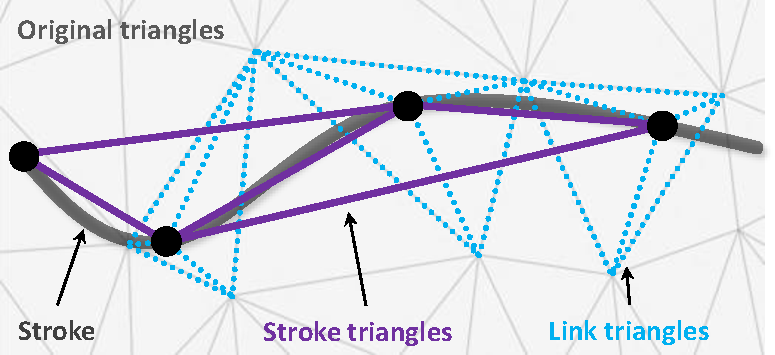
\includegraphics[width=0.85\linewidth]{images/mesh}
	\caption{The modified mesh used for stroke-preserving mesh deformation.}
	\label{fig:mesh}
\end{figure}


Given the augmented mesh structure $\mathcal{M}=(\mathcal{V}_0 \cup \mathcal{V}_s, \mathcal{T}_0\cup \mathcal{T}_s\cup \mathcal{T}_l)$, we formulate the stroke-preserving ARAP deformation as the following energy minimization problem: 
\begin{align}\label{eqn:deformationE}
	\min_\mathcal{M} \ E_0 + \beta E_{link} + \gamma E_{sketch},
\end{align}
where $ E_0 $ is the deformation energy of the original mesh $ \mathcal{M}_0 $; $ E_{link} $ and $ E_{sketch} $ are the deformation energy terms of the newly constructed triangle sets $\mathcal{T}_l $ and $\mathcal{T}_s $, respectively. 
Specifically, following \cite{Igarashi:2005}), for each triangle set, we have:
\begin{align}
 E(\mathcal{T}) = \sum_{t\in \mathcal{T}} \sum_{v_i, v_j \in t} \|\overrightarrow{v'_iv'_j} - H\overrightarrow{v_iv_j}\|^2 ,
 \end{align}
  where $ H $ is a rigid transformation matrix that is achieved by a two-step optimization algorithm; please refer to \cite{Igarashi:2005} for more details.
The same definition of $E(\mathcal{T})$ is applied to $\mathcal{T}_0, \mathcal{T}_{link}, \mathcal{T}_{sketch}$.
 Minimizing $ E_{sketch} $ keeps the shape of the strokes while minimizing $ E_{link} $ transfers the deformation of the original mesh to the strokes. 
In our system, we set the weight $ \beta $ to be a small value of 0.01, as we allow the triangles in the link triangle set to be distorted to balance between deformation and sketch shape preserving. We set $ \gamma = 1$ by default in order to better preserve the sketch shape. 
For all the strokes that need to be more rigid, we increase the corresponding $\gamma$ value by a factor greater than one. The local rigidity brush is also accumulative so the more the user brushes, the more rigid that the underlying sketch strokes will be. 

%{\bf User-specified local rigidity.} 
%The energy defined in Equation~\ref{eqn:deformationE} applies the same shape preserving weight $\gamma$ to all sketch strokes.


%\Jue{An example is shown in the accompanying video.}

\begin{figure}
	\centering
	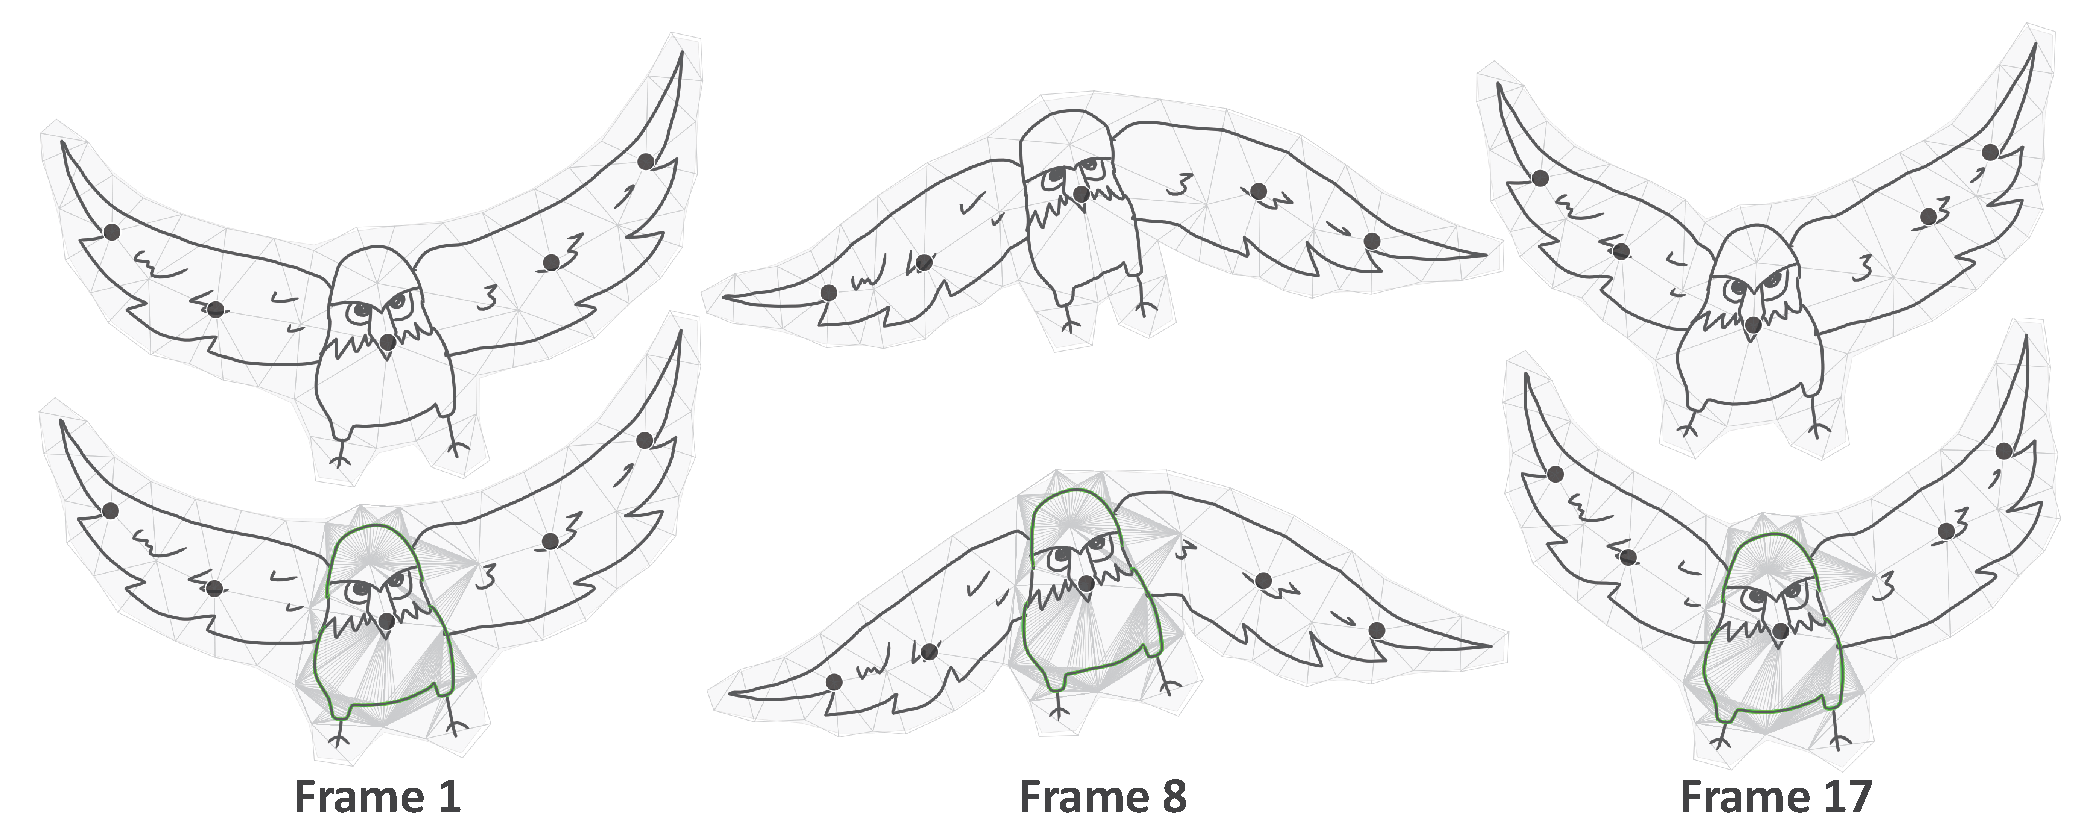
\includegraphics[width=\linewidth]{images/deformation}
	\caption{Sketch deformation results with (bottom) and without (top) applying the shape preserving method described in Sec.~\ref{motion_transfer}. The stroke in green is set to be more rigid.}
	\label{fig:deformation}
\end{figure}

\if 0
\subsection{Extensions}

\sout{
To reuse the extracted motion, we also extend it for sketches that are not similar to video objects. The main goal is to map the original key points of the video to the new sketch. This could be solved by finding the matching between the original sketch and the new one. 
We first obtain the sketch contours, $ s_o, s_n $, of the original and new sketches using the method in \ref{motion_extraction}. Then we sample $ k_0 $ and $ k_n $  points, $ \textbf{P} = \{p_i\} $ and $ \textbf{Q} = \{q_i\} $, inner the two contours. Then the correspondence could be obtained by finding the affine transformation $ T $ between the two point sets by ICP point matching methods. Then for any point $ x_o $ inner $ s_o $, we could find the corresponding position $ x_n $ inner $ s_n $ by   Given a key point's position of the first frame, $ x_i $, we first compute $ k $ nearest points in $ P $ and its corresponding points in $ \textbf{Q} $. Then the corresponding position $ x_n $ could be computed by the berry centric weight of the $ k $ points of $ \textbf{Q} $. If $ x_n $ is located outside of $ s_n $, then we remove one point from the $ k $ points and re-compute the position until $ x_n $ is located inside of $ s_n $. }
\fi

\subsection{Multiple-Layer Animation}\label{sec:multi-layer_animation}

As discussed earlier, single layer, mesh-deformation-based animation cannot handle topology change, which is common for dynamic objects (see Fig.~\ref{fig:multilayer}a). 
To handle such cases, our system allows the user to create animations with multiple layers. 
Using this tool, the user first divides the sketch strokes into several groups, each representing a layer (Fig.~\ref{fig:multilayer}b).
To avoid detaching different layers from each other in the animation, our system then automatically detects the intersections of these layers, and adds one {\em joint point} at the center of each intersection region (Fig.~\ref{fig:multilayer}c, blue circles). 
%The system then moves layers in each animation frame to make sure that the layers still attach at the joint points. 
%Our system automatically adds a joint for any two partially-overlapping layers, which is the center of the overlapping area. 
During the motion transfer stage, we first deform each layer individually based on their control points, and then re-connect meshes of layers based on the joints, as shown in Fig.~\ref{fig:multilayer}d-e. 
\begin{figure*}
	\centering
	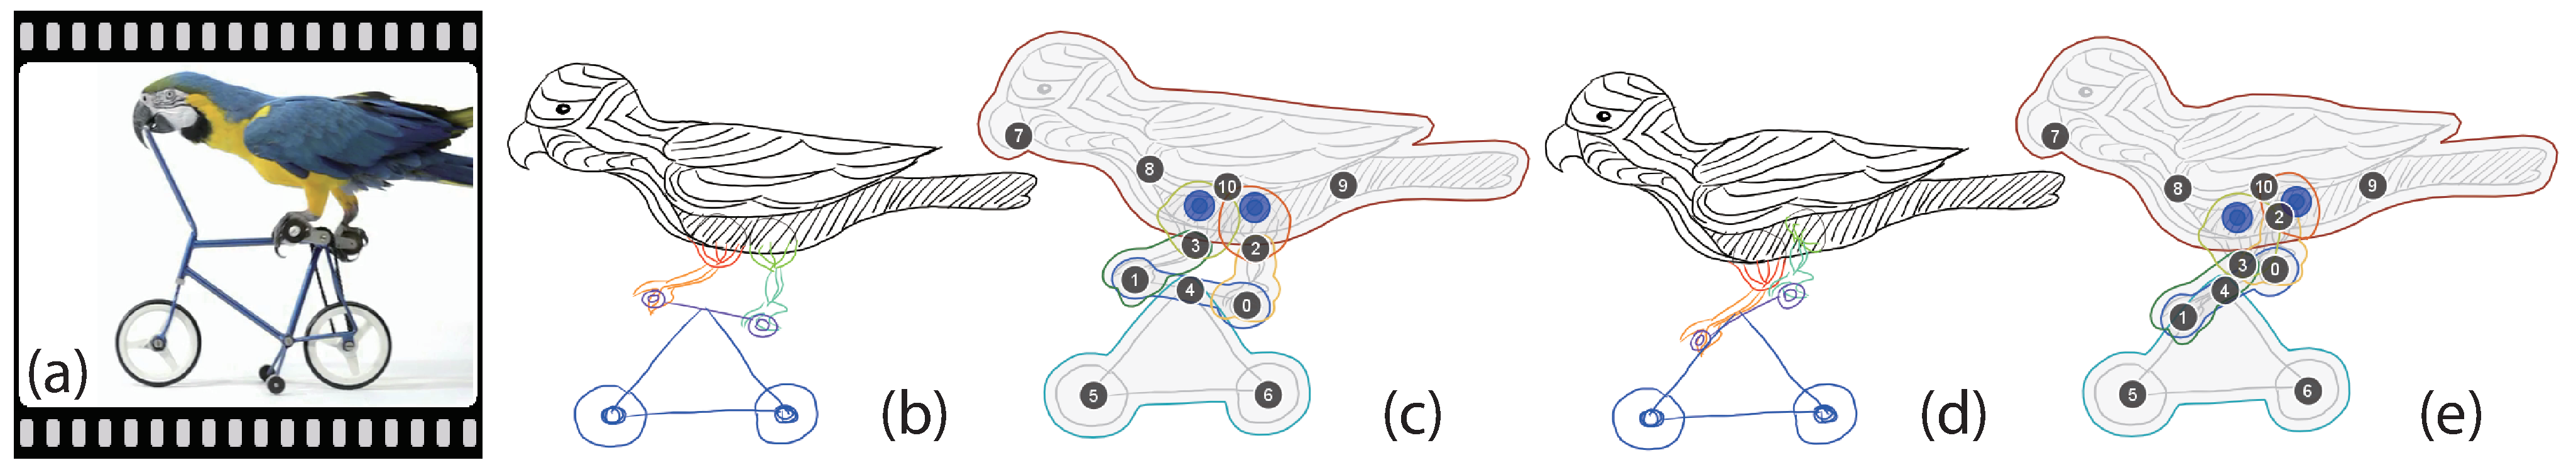
\includegraphics[width=\linewidth]{images/multilayer2}
	\caption{Multiple layer animation to handle self-occlusion and topology change. When the two legs of the macaw cross, they  introduce severe occlusion and topology change that cannot be handled by a single mesh layer. Our system allows the user to decompose the mesh into multiple layers (shown in different colors) to properly handle it. (a) Input video. (b) Grouping strokes into layers, visualized in different colors. (c) Control points and layer joints (blue circles). (d-e) Deformed sketch and new point layout in another frame.}
	\label{fig:multilayer}
\end{figure*}

%Our system aims at providing the user with an easy way to add 3D strokes to an existing shape for communicating conceptual design ideas. Strokes drawn by a user over an existing 3D shape are generally of two types. The first type lie on an existing surface. The 3D information for such a stroke can be determined easily by projection onto the surface. The second type of strokes are drawn to specify a non-existent part of the shape, indicating how the original shape is to be modified. Determining the 3D information for this type of stroke is nontrivial. Our system focuses on providing an interface to draw sketch strokes of the second type.

%We will conduct a user study to evaluate our system. The user study will consist of two parts. In User Study I, a number of participants will be invited to use both our system and an existing state-of-the-art keyframe method such as Adobe Animator to create two animations for every given pair of sketch and video. 
%To evaluate the efficiency of our system, 
%%In this experiment, the participants will be asked to create a sketch animation to a given video. 
%we will compare the completion time and the number of operations which include the sketching operations and the editing operations. 
%The participants will also be asked to answer a questionaire on the usability of our system. 
%
%The sketch animations created using the two methods will then be evaluated by a different group of participants in User Study II.
%We will ask the participants to score each sketch animation created in User Study I on aesthetics, completeness, etc. 


%\begin{figure}
%	\centering
%	\includegraphics[width=0.9\linewidth]{images/trackingcomparison}
%	\caption{}
%	\label{fig:trackingcomparison}
%\end{figure}

% Please add the following required packages to your document preamble:
% \usepackage{multirow}
%\begin{table*}[]
%	\centering
%	\caption{My caption}
%	\label{my-label}
%	\begin{tabular}{l|cc|cc|cc|cc|cc}
%		\hline
%		\multirow{2}{*}{} & \multicolumn{2}{c|}{\textbf{OURS}} & \multicolumn{2}{c|}{\textbf{STRUCK}} & \multicolumn{2}{c|}{\textbf{SPOT}} & \multicolumn{2}{c|}{\textbf{SAMF}} & \multicolumn{2}{c}{\textbf{DT}} \\
%		& \textit{Err.}    & \textit{Pre.}   & \textit{Err.}     & \textit{Pre.}    & \textit{Err.}    & \textit{Pre.}   & \textit{Err.}    & \textit{Pre.}   & \textit{Err.}  & \textit{Pre.}  \\ 
%		\textbf{Candle}   & 0.999            & 0.982           & 36.451            & 0.675            & 13.439           & 0.786           & 28.552           & 0.737           & 35.962         & 0.615          \\
%		\textbf{Cartoon}  & 1.806            & 0.940           & 3.731             & 0.884            & 7.206            & 0.759           & 5.217            & 0.801           & 7.397          & 0.744          \\
%		\textbf{Fish}     & 3.537            & 0.820           & 13.600            & 0.587            & 25.516           & 0.179           & 43.196           & 0.434           & 43.525         & 0.345          \\
%		\textbf{Kangaroo} & 4.574            & 0.805           & 12.598            & 0.666            & 19.727           & 0.427           & 44.419           & 0.282           & 21.830         & 0.415          \\
%		\textbf{Kite}     & 6.534            & 0.727           & 21.293            & 0.465            & 9.435            & 0.618           & 13.159           & 0.663           & 28.399         & 0.404          \\ \hline
%	\end{tabular}
%\end{table*}
%\qingkun{To-Do}
%We will extend the basic \textit{Live Sketch} to two applications.
%%	\textbf{Many-to-one motion transfer}
%Segmenting a character into meaningful parts or layers and animating them separately is common in animation creation. Similarly, our system will also allow transferring motions from multiple videos to different parts of a single sketch. Independent motion transfer for each part will lead to spatial inconsistency, which can be solved by existing motion retargeting method such as AniMesh~\cite{Jin:2015}.
%Another way to increase the usability of motions is to transfer motions to a sketch in different temporal intervals.  We will need to address the issue of smooth transitions between motions.
%Note that in such scenarios the number of control points used in the two motions may be different but the original mesh is the same as
%the two motions are transferred to the same sketch. 
%%the two sets of control points positions between the two control point sets at the transition position may not be well aligned and may locate at different parts of the sketch. 
%A possible solution to attain smooth transition from motion A to motion B is as follows (see Figure 6). We first compute the position of each control point of A on B's deformed mesh by mesh interpolation. Next we can find a new motion trajectory for each point of motion A during B's time interval. A smooth transition trajectory can easily be found between the two trajectories by Hermite 
%interpolation.
%by Laplacian smoothing after connecting them. 
%Similarly, we can obtain a smooth transition trajectory for each control point of motion B. Therefore, the animation can be transited smoothly based on the transition trajectories.

%Interactive illustrations can provide a more playful or informative experience~\cite{Kazi:2014b}. We will also extend our \textit{Live Sketch} tool to achieve dynamic interactive animations. Users can interact with the animation to control its playback direction, speed of playing and locally deform near a dragged point. 
%We will provide a user interface that when the user drags one part of the sketch, the animation will be played forward or backward according to the drag direction with respect to the nearest motion trajectory. The speed of playing will depends on the cursor speed.  The point on the sketch where it is being dragged will be deformed such that it stays attached to the cursor. This can be achieved by applying a sketch deformation method described in Task D, where the drag point is treated as an additional control point.
%% (user is also required to give another static point). 
%Different dynamic motion constraints can also be specified to different parts, for example, producing the effect of magnifying the motion of certain parts while suppressing the motion of the other parts. 
%Furthermore, dynamic dragging constraints can also be applied to simulate effects such as flowers being blown by wind.  

%It also allow user to add an external force like wind with dynamic direction and speed.
%We provide a user interface that when user drag some part of the sketch, the animation would be played adaptively and dynamically and also respect to user's dragging position. The animation speed and direction can be computed by the dragging speed and direction. To make sure that the dragging part is always attached to the cursor, a sketch deformation is applied to the deformed sketch using the method in Task D, where the dragging point is treated as the control point (user is also required to give another static point). Furthermore, our system can also produce dynamic animation when user specifies dynamic dragging constraints such as the wind, or highlights the motion of some parts by magnifying its motion and reducing others'.

%
%\subsection{Extensions}
%
%Our tool aims to animate a sketch using the same motion of the object in the video, it thus will look as real as in the video. Since the users might want to produce a stylized animation, we will provide post-animation stylization tools, such as using animation filters~\cite{Wang:2006}, applying the 12 animation principles~\cite{Kazi:2016}, and adding animation looping.
%
%%{The methodology described above focuses on motion transfer for a single object.} An extracted motion can also be re-used and transferred to multiple objects.  In that case, motion re-targetting is necessary. 
%
%%We will also investigate creation of sketch animations containing numerous objects. For this purpose, we will need to design and implement a new user interface that can combine the results of several animation results of our method into one scene.
%
%Sketching on touch-based devices is direct and natural. Hence,
%implementing Live Sketch on devices like iPad and iPhone will be highly desirable.  This will require redesigning the user interface to improve user experience on sketching and interactions, such as integrating multitouch features and stylus pen.

%In our system, we require only coplanar strokes be drawn in each step. This setting ensures that our system is able to generate the expected 3D sketch with only simple interaction. However, this restriction may hinder the user during drawing. The ultimate goal of allowing the user to draw strokes on arbitrary planes or surfaces in any order is too difficult. Instead, we will further investigate how to make our system more general by introducing other type of constraints besides the coplanar constraint for drawing strokes, constraining the current set of drawn curves to be on a curved surface, or to be symmetric. 
%%\ca{Similar to the current algorithm, we will borrow the geometry information to constrain the drawn curves. Specifically, 
%If the matched sharp edges are on a common curved surface that is extracted from the shape, the surface is a potential canvas. If the drawn strokes are self-symmetrical after an affine transformation, the canvases that realize this transformation might be desirable ones. When the user draws a set of strokes, it is unknown which constraint should be used. A possible solution will be to traverse all the constraints and generate all possible candidate 3D strokes which will be ranked using the same criteria described before.

%An issue to solve then would be how does the system automatically recognize what type of constraint to enforce on the drawn strokes. \ca{Possible solutions? curved surface derived from the given shape}

%Man-made shape is the main focus of our system. It is because designing man-made shapes is more common than organic shapes. 
%For example, the user may want to modify the design of an existing furniture model, or change the appearance of a building model. When designing a 3D scene, the models in this scene are mostly man-made. In our system, we will mainly focus on the following information.




%\section{Methodology}
%The pipeline of our system is shown in Fig~\ref{overview}. Given two inputs sketch and the video, our method contains three main steps to animate the static sketch $ \mathcal{S} $:
%
%\begin{description}
%	\item[Video\&Sketch Alignment.] Alignment between the sketch (vector graphics) and video frame (bitmap image) is very hard. We proposed a method that extracts the feature points both good to track in video and in the region of user's interest in sketch.
%	\item[Motion Extraction.] Drifting problem is always hard to avoid in video tracking, which could produce unexpected animation results. We present a   tracking method that keeps the object structure even when some parts drifts at some frames.
%	\item[Motion Transfer.] With the correspondence and the extracted video motion, we animate the sketch using a stroke-preserving as-rigid-as possible mesh deformation method. This method could keep the stroke shape well even with large deformation. 
%\end{description}
%
%\begin{figure*}[t]
%	\centering
%	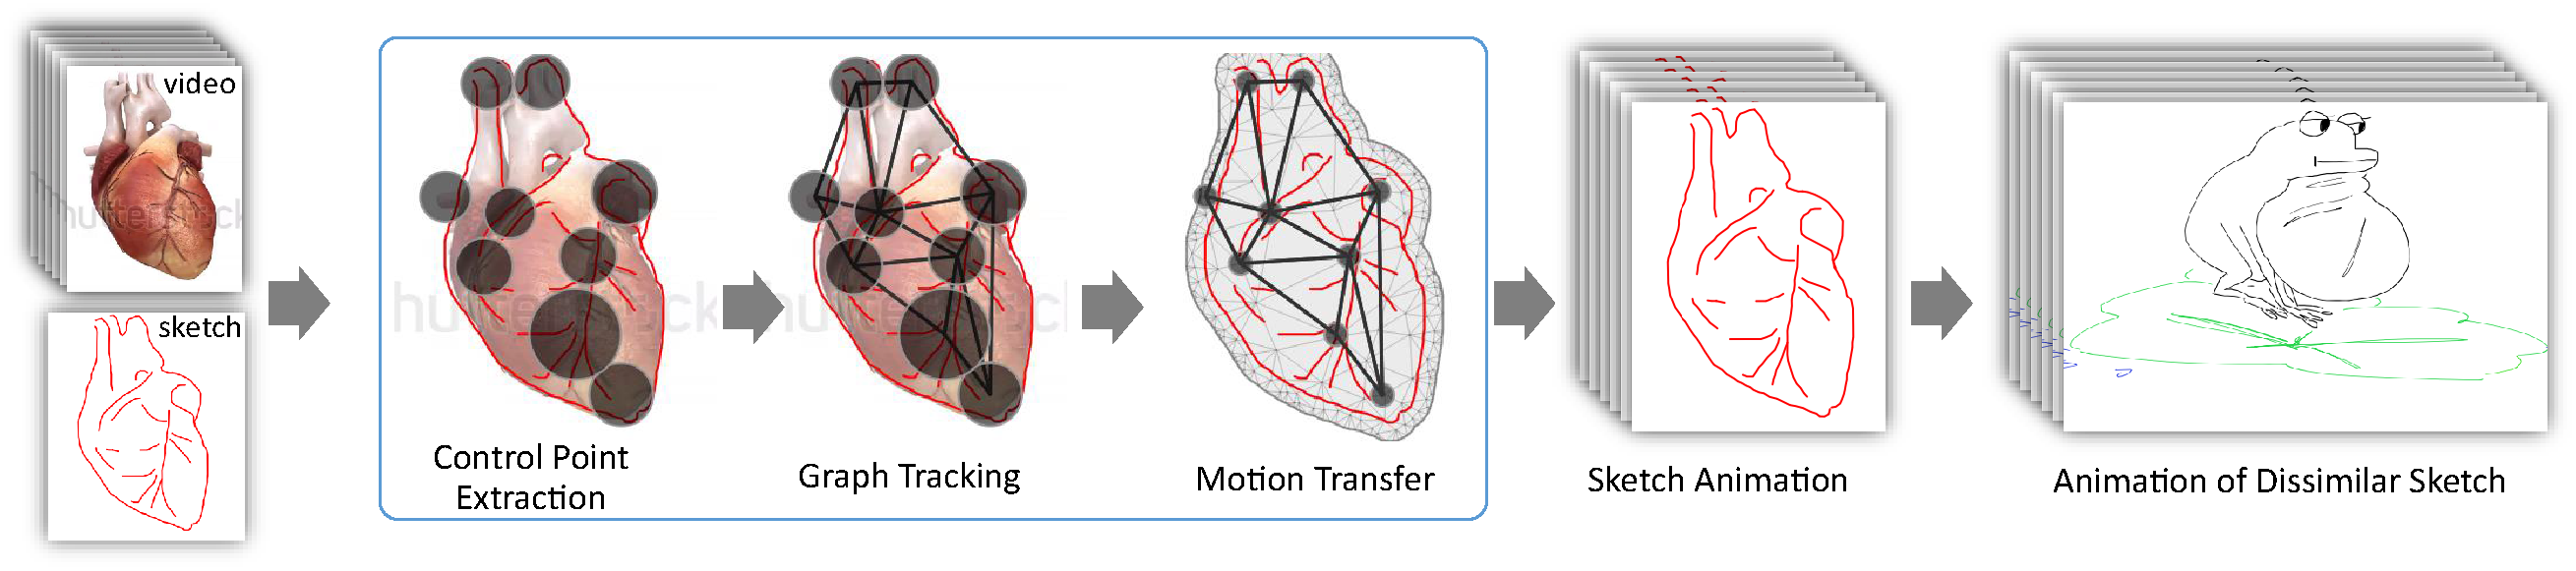
\includegraphics[width = 0.95\linewidth]{images/overview}
%	\caption{Given the sketch and the video, the first step alignment would try to extract some good feature points from video and sketch and compute their correspondence.
%		Then we extract the motion by tracking the good feature points of the video by using object structure.		
%		Combined with the correspondence and the motion, we used a stroke-preserving ARAP method to transfer the motion to the sketch.
%		After the three steps, the final sketch animation is generated. 
%	}
%	
%	\label{fig:overview}	
%\end{figure*}
%
%\subsection{Video\&Sketch Alignment}\label{alignment}
%Finding the correspondence between video and sketch is tough problem, because the latter is more abstract and semantic. Therefore, we need to extract the feature points that are both good to track for video and good to control for sketch.
%
%We first extract the good feature to control for sketch and to track of the first video frame by scale irrelevant corner detection method[XXX]. Then a graph matching is used to find the best one-to-one mapping between the two feature point set [XXX].
%
%However, sometimes it would be hard or even impossible to detect the correspondence, because the sketch and the video object do not have similar structure (see the example in Fig. [XXX]). we also provide a user interface to edit the flexible correspondence. 
%
%\begin{figure}
%	\centering
%	\includegraphics[width=0.85\linewidth]{C:/Users/suqin/Documents/flexible}
%	\caption{}
%	\label{fig:flexible}
%\end{figure}
%
%
%\subsection{Motion Extraction}\label{motion_extraction}
%The goal of this step is extract robust motion for each feature point that is extracted in previous step. We proposed a method that could 
%1)track the object that could preserve its structure 2) keep the structure by using the structure even if drifting problem happens at some parts.
%Unlike previous graph-based or structure-preserving object tracking methods, our method could detect the drifting parts and predict its positions by spatial and temporal neighborhood.
%Our structure preserved object tracking method mainly considers two part: 1) $ E_t $ appearance energy that existing tracking methods 2) $ E_s $structure energy that measures the structure deformation. Assuming that we could obtain several candidates for the $ i $th part, $ \{ c_{ij} \} $ ($ c_{ij} $ is contains the candidate position $ p_{ij} $ and same size with initial frame), with appearance energy ascending order. So this could be formulated as a energy minimization problem
%\[ E* = \min_{C \in \mathcal{C}} E_t(C) + \alpha E_s(C) \]
%over all candidate configurations in $ \mathcal{C} $, where $ E_s = \sum_{e} \Delta d + w\sum_{\theta} \Delta \theta$ is measured by the edge length and angle difference regarding to initial object position.
%
%However, 1) it requires searching exponentially many configurations; 2) some candidates may break the structure even if they may have small appearance energy. To solve this problem, we will propose a method that could detect the bad candidates, preserve the global structure by the good ones and then predict the positions by its spatial and temporal neighborhood.
%
%%\begin{algorithm}
%%	\caption{Motion Extraction}\label{euclid}
%%	\begin{algorithmic}[1]
%%		\Procedure{MyProcedure}{}
%%		\State Initialize: $ C^* \gets (c_{11}, c_{21}, ..., c_{i1}, c_{n1}) $
%%		
%%		
%%		\While {true}
%%		\State $ i^* \gets \max_i E_t(C^*_i) + \alpha E_s(C^*-C^*_i) $
%%		\State $ j^* \gets \min_j E_t(c_{i^*j}) + \alpha E_s(C^*-C^*_{i^*} + c_{i^*j}) $
%%		
%%		\EndWhile
%%		
%%		\State $\textit{stringlen} \gets \text{length of }\textit{string}$
%%		\State $i \gets \textit{patlen}$
%%		\If {$i > \textit{stringlen}$} \Return false
%%		\EndIf
%%		\State $j \gets \textit{patlen}$
%%		\If {$\textit{string}(i) = \textit{path}(j)$}
%%		\State $j \gets j-1$.
%%		\State $i \gets i-1$.
%%		\State \textbf{goto} \emph{loop}.
%%		\State \textbf{close};
%%		\EndIf
%%		\State $i \gets i+\max(\textit{delta}_1(\textit{string}(i)),\textit{delta}_2(j))$.
%%		\State \textbf{goto} \emph{top}.
%%		\State \Return $ C $
%%		\EndProcedure
%%		
%%	\end{algorithmic}
%%\end{algorithm}
%
%\subsection{Motion Transfer}\label{motion_transfer}
%
%Motion transfer aims to transfer the extracted motion of video to the sketch by using the extracted correspondence in section \ref{motion_extraction}. The simplest way is using as-rigid-as possible(ARAP) mesh deformation method.
%To generate the mesh that is used to deform the sketch, we triangulate the contour that is obtained by active contour method for the sketch image. Then we can animate the sketch by deforming the mesh with the feature points' position as handles. However, ARAP mesh deformation could not preserve the stroke shape because it only keeps the rigidibility of the mesh triangles (see the example in Fig.XXX). 
%
%Therefore, we proposed stroke-preserving ARAP method to preserve the stroke shape during the mesh deformation.
%Denote the feature positions of the $ t $th and $ (t + 1) $th frame as $ \mathbf{p}^t = \{p^t_{i}\} $ and $ \mathbf{p}^{t+1} = \{p^{t + 1}_{i}\} $.
%To preserve the stroke shape, we reconstruct the original mesh $ \mathcal{M}_0 = (\mathcal{V}_0, \mathcal{T}_0) $ by adding one vertex set $ \mathcal{V}_s $ that includes all the sketch points and two triangle sets $ \mathcal{T}_s, \mathcal{T}_l $, where
%
%\begin{description}
%	\item[Sketch triangle set $\mathcal{T}_s $] is constructed by connecting every three consequent points on each stroke;
%	\item[Link triangle set $\mathcal{T}_l $] is constructed by connecting each sketch point with its outer triangle�s vertices.
%\end{description}
%
%\begin{figure}[t]
%	\centering
%	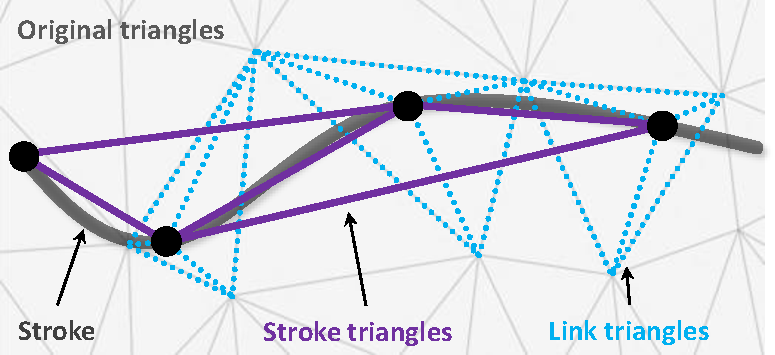
\includegraphics[width = 0.95\linewidth]{images/mesh}
%	\caption{Reconstructed mesh for stroke-preserving ARAP deformation.}
%	
%	\label{fig:mesh}	
%\end{figure}
%
%Then, the ARAP mesh deformation is applied to the new constructed mesh $ \mathcal{M} = (\mathcal{V}, \mathcal{E}) $ where $ \mathcal{V} = \mathcal{V}_0 \cup \mathcal{V}_s $ and $ \mathcal{E} = \mathcal{E}_0 \cup \{e|e\in \mathcal{T}_s \cup \mathcal{T}_l\} $ by the following energy minimization formulation:
%\[ \min E_0 + E_{1ink} + \beta E_{sketch} \]
%, where $ E_0 $ is deformation error of the original mesh $ M_0 $, $ E_{1ink} $ and $ \beta E_{sketch} $ represents the error of the new added triangle sets $\mathcal{T}_s $ and $\mathcal{T}_l $. The main idea of this method is that the original mesh will try to deform the sketch triangles through the intermediate link triangles. If the weight of the stroke triangles are large enough, the shape of the stroke would be preserved. $ \beta $ is set to be 10 in our implementation.



\begin{figure*}
	\centering
	\includegraphics[width=\linewidth]{images/result3}
	\caption{Some results produced by our system. From left to right: the first frame of the video, the extracted motion trajectories, the corresponding animation control points and several frames of the final animation. Column 1: input video. Column 2: tracking points and their trajectories. Column 3: control points, strokes with rigidity constraints (green) and layer joints (blue). Other columns: animation results. }
	\label{fig:results}
\end{figure*}


\section{Results}\label{sec:results}

We have implemented our system in C++, and tested it on  a wide variety of input sketch drawings and videos. Our method can handle complex non-rigid motions well, e.g., elastic motion (Fig.~\ref{fig:results}a), articulated motion (Fig.~\ref{fig:results}c) etc.
By applying layered-animation, it can also produce high quality animation that involves self-occlusion (Fig.~\ref{fig:results}c).
 The motion extracted from one video sequence can be easily reused to drive different input sketches with different styles (Fig.~\ref{fig:teaser}; Fig.~\ref{fig:results}b; Fig.~\ref{fig:tasks}). Similarly, multiple motion examples can be applied to different parts of a single complex drawing to create spatially complex animations, as shown in Fig.~\ref{fig:results}d, where the final animation combines the extracted motion from the virus and kite videos. Please refer to the accompanying video for the input videos and resulting animations. 
 
% All the input videos and resulting animations of these examples can be found in the accompanying video. 

\section{Evaluations and Discussions}\label{sec:evaluation}

We conducted a pilot study to evaluate the efficiency and effectiveness of our system. While there exist professional animation software such as \emph{Adobe Flash} and \emph{Toon Boom Harmony}, directly comparing with them is not easy, as our system is designed for users with a wide range of skill sets while those tools are mainly designed for animation professionals due to the involved steep learning curve. Instead of comparing with these tools, we are thus interested more in exploring whether our system can be used effectively by users both with and without adequate animation skills. We are also interested in knowing if our system can fully support users' creativity to animate sketches with a wide range of styles. 
We thus designed two pilot studies to address these two questions. 

\subsection{Pilot Study I}
\begin{figure}
	\centering
	\includegraphics[width=\linewidth]{images/tasks}
	\caption{The tasks used in Pilot Study I. Row 1: the input videos; Row 2\&3: the two sketches to be animated.}
	\label{fig:tasks}
\end{figure}

{\bf Participants and Apparatus.}  12 university students (a1 to a12) were invited to participate in this study, including {6} male and {6} female. % The ages of the subjects ranged from xx to yy. 
Half of the subjects (a1-a6) had good to professional drawing skills and 2D animation skills, while the other half had no or very little animation experience. All subjects were enthusiastic about the idea of creating their own 2D animations. 
%
A touch-screen notebook (Surface Pro 4 with Intel(R) Core(TM) i5-6300U @2.40GHz 2.5GHz 8GB RAM) running Windows 10 was used as the testing device. Our system runs smoothly at an interactive rate on this device.

{\bf Design and Procedure.} In the study each participant was first given a 20-minute training on how to use our system to extract and transfer motion, instructed by one of the authors.
The subjects were then given 10 minutes to practice using the same example. 
After the subjects felt comfortable moving forward, they were asked to create animation for 5 different examples {(namely, bird, virus, fish, heart, and kite)}, each including an input video and two given sketches of different characters (Fig.~\ref{fig:tasks}). In this part of the study, input sketches were given to the participants, since we wanted to focus on evaluating the usability of motion extraction and transfer. No time limit was set for this task, and one of the authors was always available to answer any questions the subjects might have. 

%For the motion extraction part, user first loads a video in to the system for motion extraction. An empty motion will be created and put in the source motion list. User can add a tracking point at any positions of any frame and correct its position if necessary. The motion trajectory of a selected point is also visualized to the user for a global preview of its motion.

%After motion extracted, user can switch to the animation mode to do motion transfer. User just loads one of the given two sketch into our system. The it will be animated after user double clicking the extracted motion in the source motion list. User can edit (move/delete) the animation control points, or add a shape constraint to any stroke.
%We also provides three extra tools. One is for fixing the position of the selected strokes so they will not be animated, which are usually the background decoration lines. The second is pin tool to add a static control point to the mesh. It is very helpful for creating a smooth motion transition between the adjacent animated lines and static lines. The third one is to control the motion magnitude (0.1-10 times) and direction($ 0-360^{\circ} $). We just provide an option to let user create some animations that have some variation with the video motion. 

%After finishing the first animation, user are required to animate the second sketch using same tools.

{\bf Results.} Our system recorded the timings of  each subject, including the start and finish times of both the motion extraction and the motion transfer steps. 
We also recorded all the user interactions: adding and adjusting tracking points; labeling decoration lines; applying local rigidity brushes, and adjusting motion scale and rotation, etc.
The statistics are plotted in Fig.~\ref{fig:userstudytime} and Fig.~\ref{fig:userstudyoperation}, and listed in Table.~\ref{table:timings}.

%In addition, the motion extraction is efficient, and user can 
% the number of tracking points adding/editing operations, control points editing operations of sketch1 and sketch2. 
The results show that there was no significant difference between novice and artist users on the user time of motion extraction and transfer. On average, novice users and artists respectively spent $3.066$ and $3.107$ seconds per frame. Both groups of subjects spent the most time on the heart example, mainly because the specification of control points for motion extraction is less obvious for elastic motion. Artists applied slightly more manual operations (on average $0.655$ operations per frame for artists and $0.510$ operations per frame for novices). This is possibly because they preferred to have a finer control on the tracking and motion results to produce higher quality animation. Interestingly, their animation experience helped them operate faster, which is perhaps the reason why their finishing times were comparable to those of the novices.

\begin{figure}
	\centering
	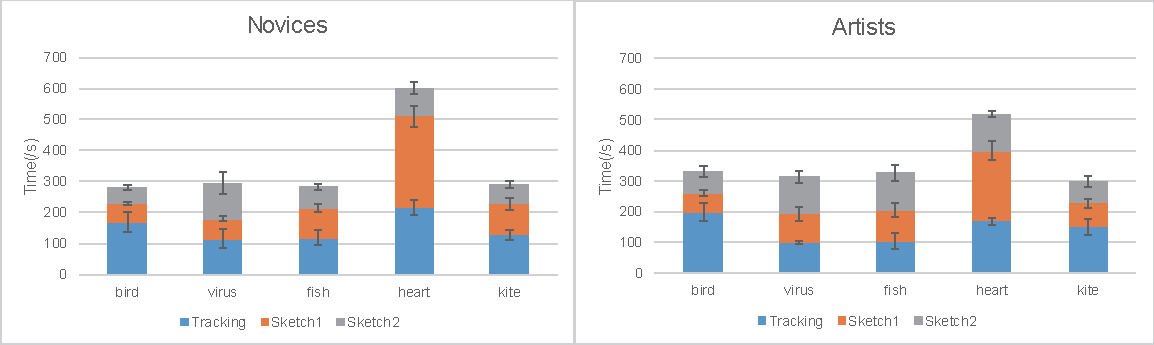
\includegraphics[width=\linewidth]{images/userstudytime3}
	\caption{Finishing time of Pilot Study I, for novice (left) and artist (right) users. Tracking: motion extraction time; Sketch1 and sketch2: motion transfer times for sketch1 and sketch2. There was no significant difference between novice and artist users.}
	\label{fig:userstudytime}
\end{figure}
\begin{figure}
	\centering
	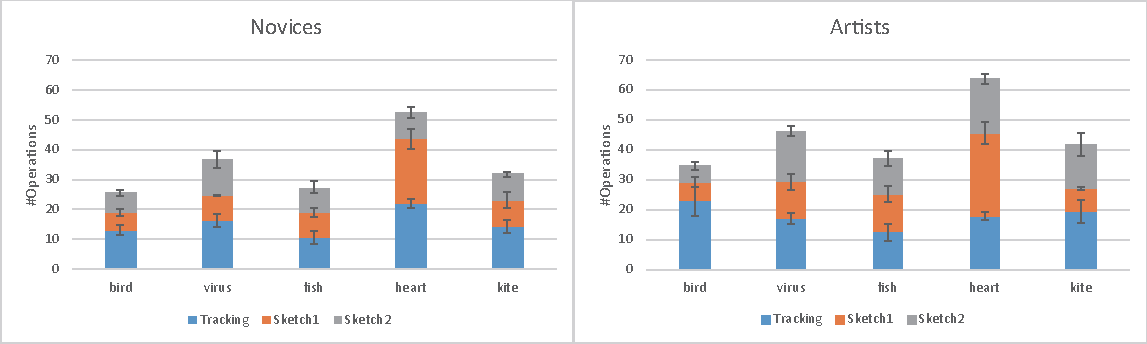
\includegraphics[width=\linewidth]{images/userstudyoperation3}
	\caption{
		The number of manual operations in Pilot Study I, for novice (left) and artist (right) users. Artists in general provided more manual operations to improve the animation quality. 	}
	\label{fig:userstudyoperation}
\end{figure}

\subsection{Pilot Study II}\label{sec:userstudy2}

In the second study, we asked the subjects who have good drawing skills (a1 to a6) from Study I to freely draw two sketches for each video used in Study I and animate them using their extracted motion in Study I. The motion could be edited or re-extracted if desired. % We then asked the user to rate the system. 
Some selected sketches drawn in this study are shown in Fig.~\ref{fig:us2sketch}, revealing a large variation both in drawing styles and in the level of details. 
The results show that our system can support users' drawing creativity reasonable well, despite using only 5 input videos.

We also collected user feedback after they finished the study, by filling out a questionnaire about their experience with both the motion extraction and motion transfer components of the system. Overall the participants were satisfied with our system. Five out of six participants mentioned the motion extraction tool was easy to learn and use. There were also five users who liked the fact that they did not need to control the animation frame-by-frame. However, four users also pointed out some limitations of the results. For example, our system might produce unexpected results when tracking points were located in smooth image regions. It also cannot produce good animation when the object of interest undergoes a 3D rotation, which is a fundamental limitation of the system as it does not know anything about 3D. 

We also asked the artists to comment on the alternative tools they might use to create such animations, and how long it would take by estimation. They mentioned a couple of commercial animation software like \emph{Adobe Flash}, \emph{Toom Boom}, but they estimated a much longer time (from one to several hours) might be needed to create similar animations with existing tools, since they would have to manually deform the input drawing or redraw it frame by frame. We are interested in conducting a more formal comparative study against these tools in the future.
 
\if 0 
\begin{figure}
	\centering
	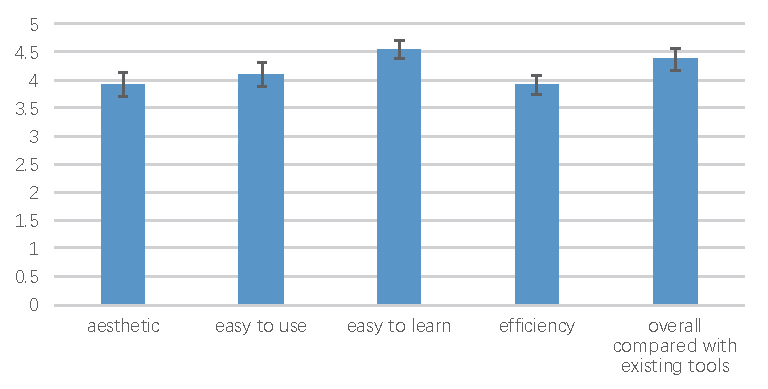
\includegraphics[width=\linewidth]{images/feedback}
	\caption{User feedback. All quantities are expressed as mean $ \pm $ standard deviation in 5 point. }
	\label{fig:feedback}
\end{figure}
\fi

\begin{figure}
	\centering
	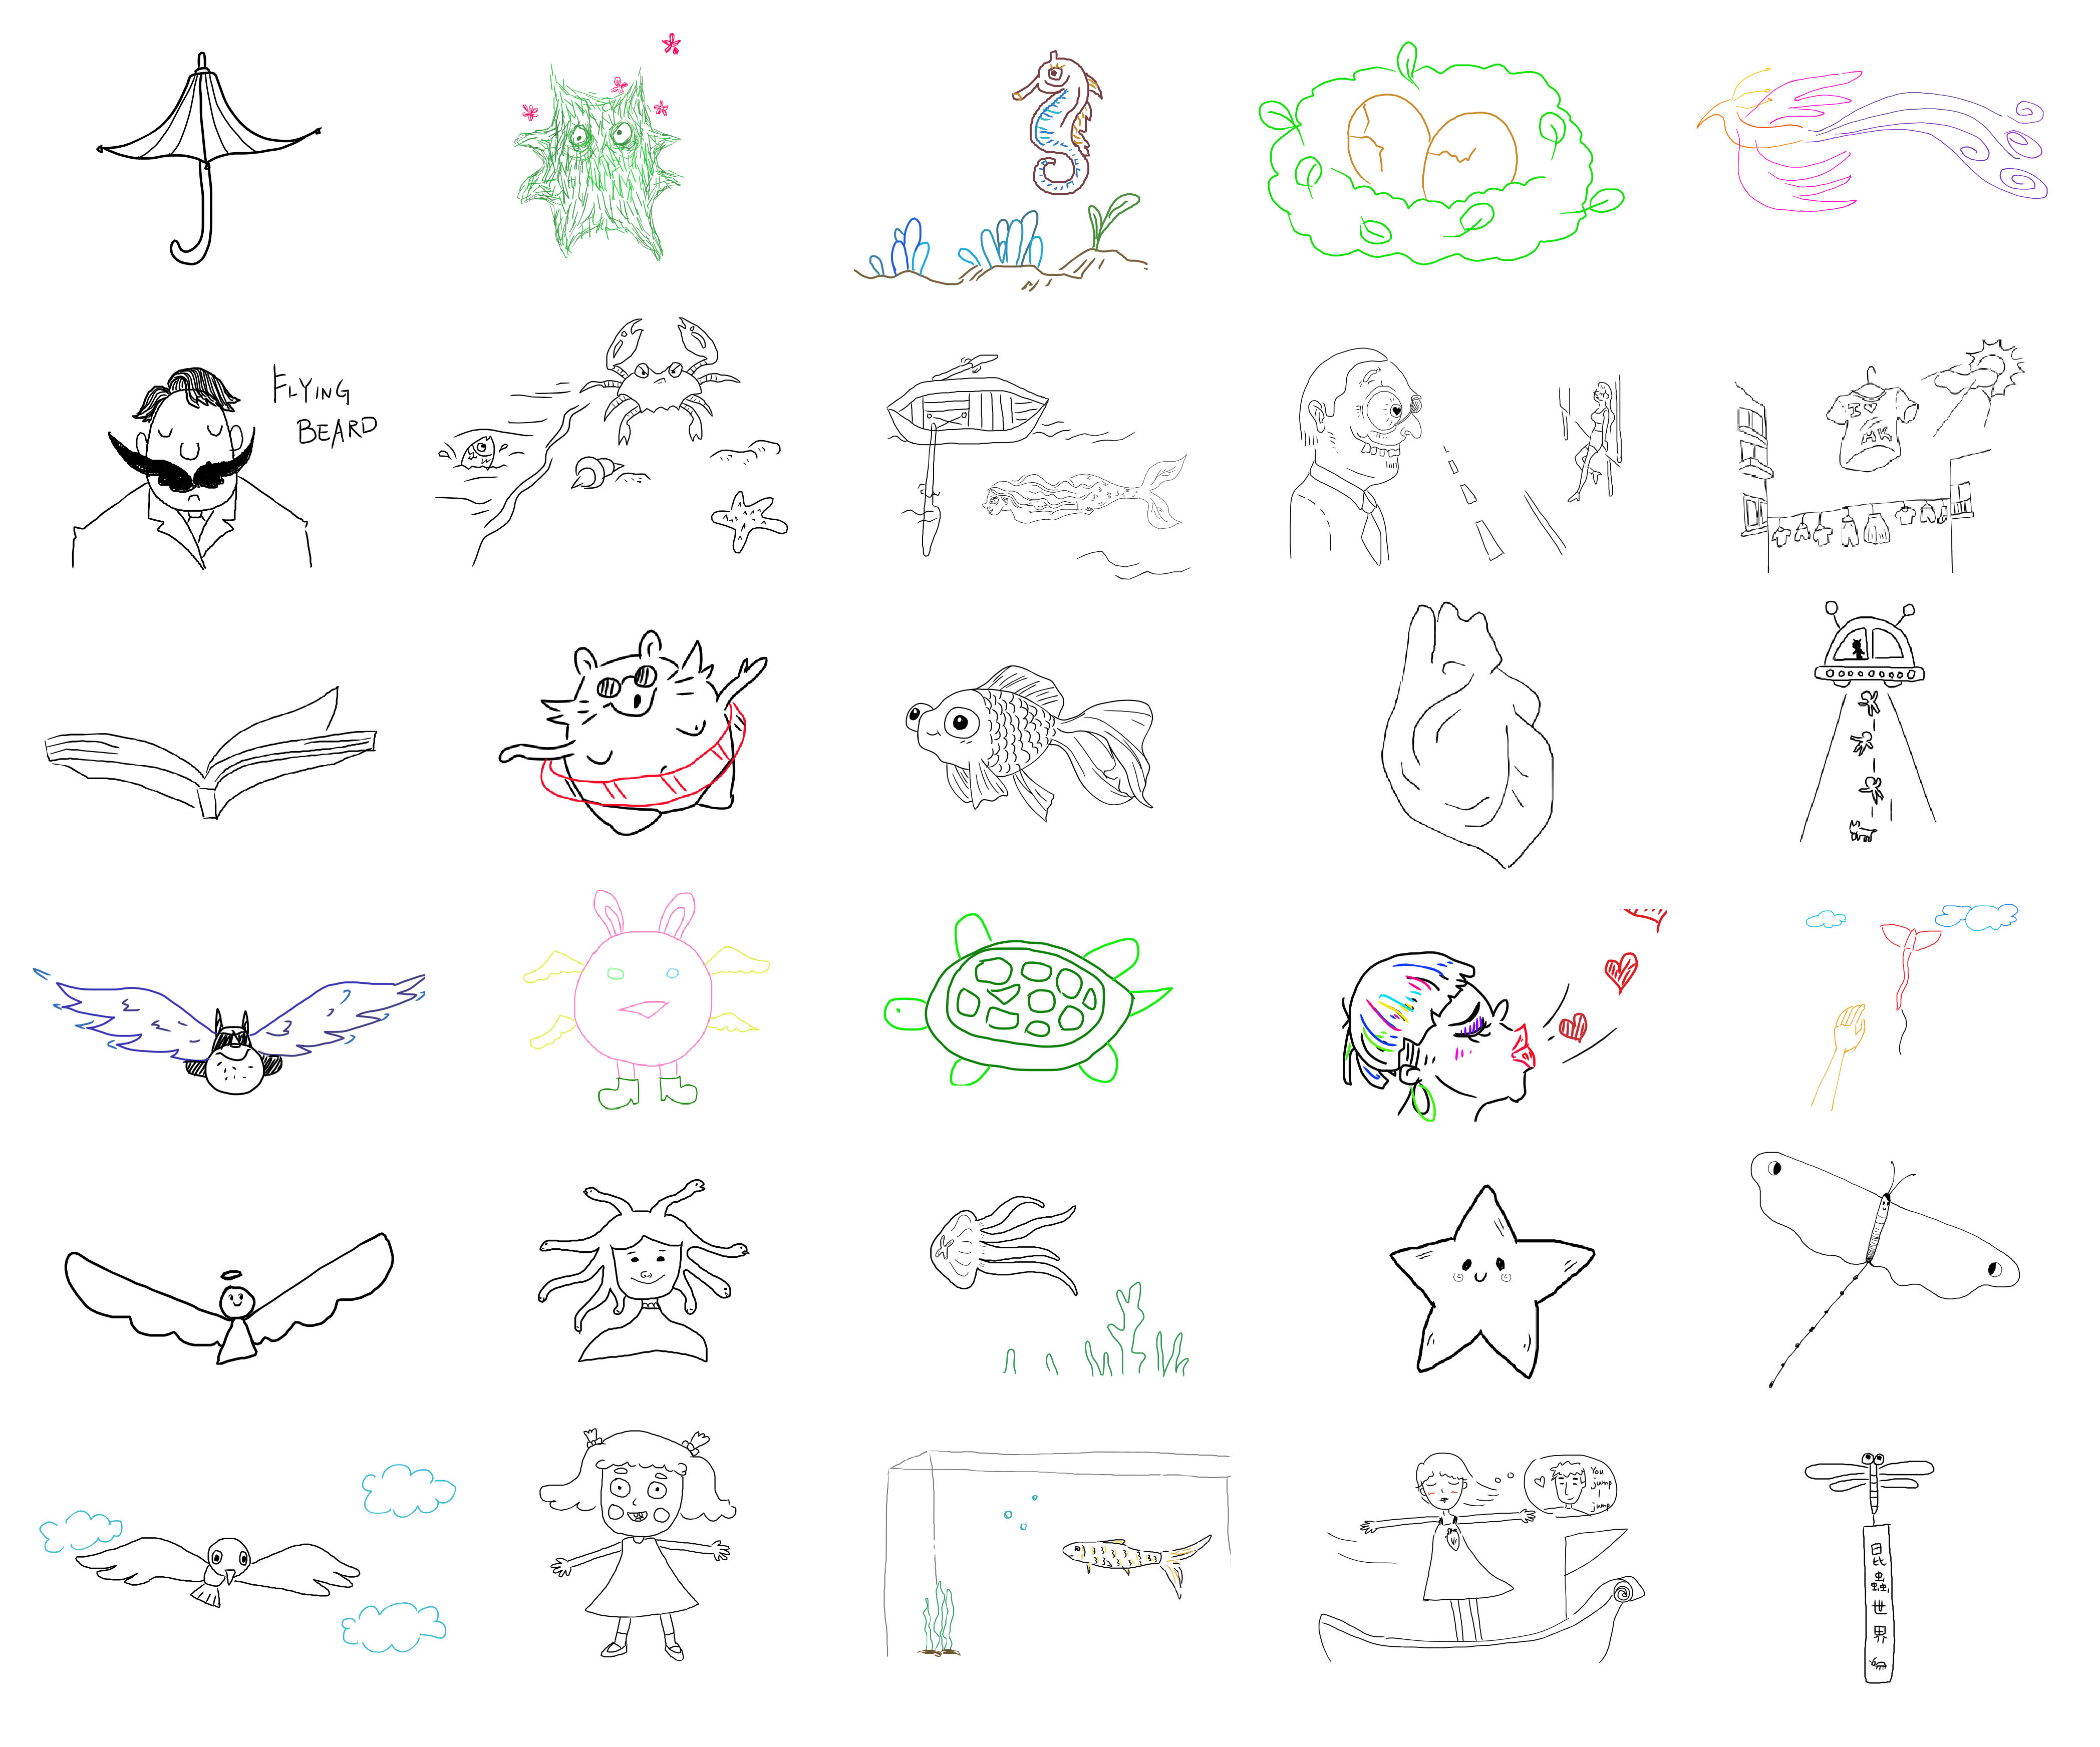
\includegraphics[width=\linewidth]{images/us2sketch2}
	\caption{Selected sketches from Pilot Study II. Each row is a collection of one artist's work. The columns correspond to the tasks in Fig.~\ref{fig:tasks}.}
	\label{fig:us2sketch}
\end{figure}

\begin{table*}[]
	\centering
	\caption{Timings of Pilot Study I. ``tracking'', ``sketch1'', ``sketch2'' refer to the average tracking time and animation time for each input sketch in seconds, respectively.}
	\label{table:timings}
	\begin{tabular}{c|c|cccc|cccc}
		\hline
		&         & \multicolumn{4}{c}{Artist}                                  & \multicolumn{4}{|c}{Novice}                                 \\ \hline
		video & \#frame & \#control points & tracking (s) & sketch1(s) & sketch2(s) & \#control points & tracking(s) & sketch1(s) & sketch2(s) \\ \hline
		bird  & 45      & 4.7      			& 198.6547     & 62.1088     & 69.89383    & 4.2         & 169.5982     & 59.1895     & 52.06267    \\
		virus & 18      & 9.5              & 100.1268     & 92.02217    & 121.385     & 8.3         & 115.0775     & 65.71083    & 114.1543    \\
		fish  & 118     & 8                & 103.3173     & 101.2937    & 121.1722    & 6.7         & 118.7607     & 94.93717    & 69.52433    \\
		heart & 31      & 8                & 168.7968     & 229.32      & 122.1046    & 10               & 217.5835     & 291.8997    & 91.66283    \\
		kite  & 129     & 4.8      			& 150.2277     & 77.24233    & 71.84567    & 5                & 128.2655     & 99.9025     & 61.71783    \\ \hline
	\end{tabular}
\end{table*}
\section{Conclusion and Future Work}

We have presented a new interactive system for animating sketch drawings using video examples. The key idea is to extract object motion presented in the video using sparse point tracking, and transfer it to the sketch image using controlled mesh deformation. For motion extraction, we propose a new tracking method that is robust against occlusion and ambiguity, and further combines it with easy user controls for reliable tracking. For motion transfer, our system allows the user to fine control the animation using a set of interactive tools.  
We conduct a user study to evaluate the usability of the system for both novice and artist users. 

We believe our current work has only scratched the surface of an exciting opportunity. As pointed out earlier, our system still has problems for handling smooth image regions such as deforming clouds, or stochastic motions such as ocean waves.  Expanding the system to handle more types of objects is always desirable. The system currently can only transfer the raw motion extracted from video, it would be interesting to combine it with previous motion stylization or exaggeration approaches, such as the Animation Filter~\cite{Wang:2006} to create even more convincing animation. We also plan to build a large motion library using our system on a large video corpus, so that motion can be automatically transferred to animate an entire drawing that contains multiple objects. 



%\section{Acknowledgments}
%
%Sample text: We thank all the volunteers, and all publications support
%and staff, who wrote and provided helpful comments on previous
%versions of this document. Authors 1, 2, and 3 gratefully acknowledge
%the grant from NSF (\#1234--2012--ABC). \textit{This whole paragraph is
%  just an example.}

% Balancing columns in a ref list is a bit of a pain because you
% either use a hack like flushend or balance, or manually insert
% a column break.  http://www.tex.ac.uk/cgi-bin/texfaq2html?label=balance
% multicols doesn't work because we're already in two-column mode,
% and flushend isn't awesome, so I choose balance.  See this
% for more info: http://cs.brown.edu/system/software/latex/doc/balance.pdf
%
% Note that in a perfect world balance wants to be in the first
% column of the last page.
%
% If balance doesn't work for you, you can remove that and
% hard-code a column break into the bbl file right before you
% submit:
%
% http://stackoverflow.com/questions/2149854/how-to-manually-equalize-columns-
% in-an-ieee-paper-if-using-bibtex
%
% Or, just remove \balance and give up on balancing the last page.
%
\balance{}

% BALANCE COLUMNS
\balance{}

% REFERENCES FORMAT
% References must be the same font size as other body text.
\bibliographystyle{SIGCHI-Reference-Format}
\bibliography{reference}

\end{document}

%%% Local Variables:
%%% mode: latex
%%% TeX-master: t
%%% End:
